% Created by tikzDevice version 0.12.4 on 2023-03-21 21:49:43
% !TEX encoding = UTF-8 Unicode
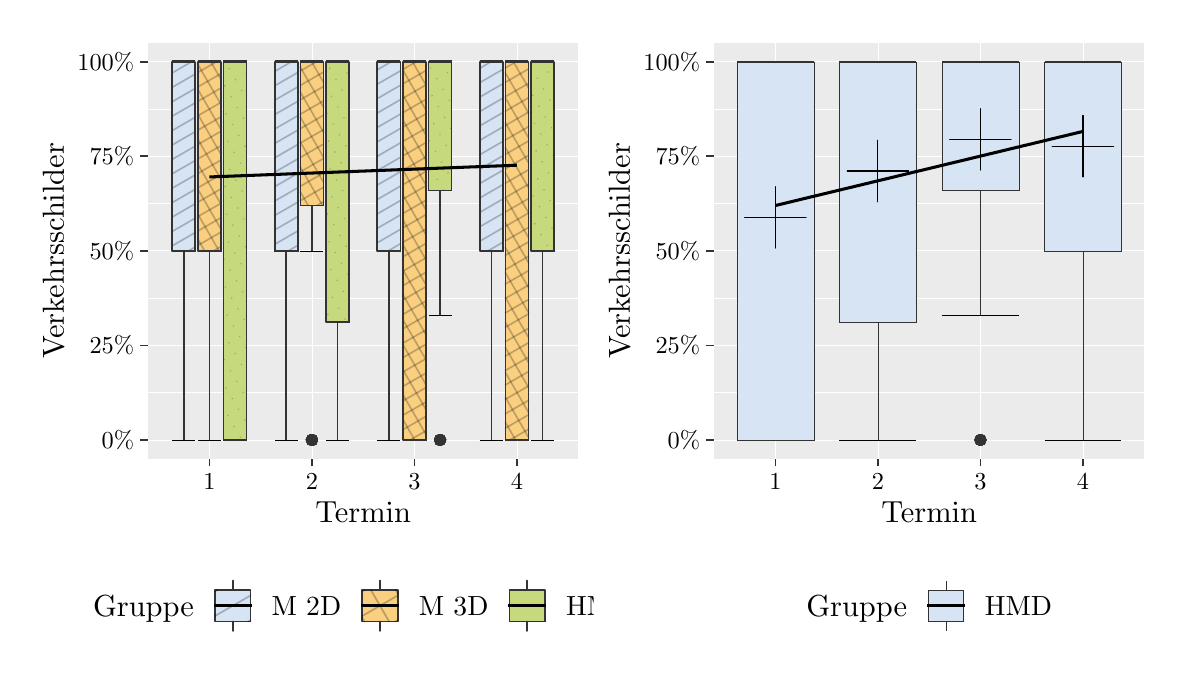
\begin{tikzpicture}[x=1pt,y=1pt]
\definecolor{fillColor}{RGB}{255,255,255}
\path[use as bounding box,fill=fillColor,fill opacity=0.00] (0,0) rectangle (409.05,231.26);
\begin{scope}
\path[clip] (  0.00,  0.00) rectangle (204.52,231.26);
\definecolor{drawColor}{RGB}{255,255,255}
\definecolor{fillColor}{RGB}{255,255,255}

\path[draw=drawColor,line width= 0.6pt,line join=round,line cap=round,fill=fillColor] (  0.00, -0.00) rectangle (204.52,231.26);
\end{scope}
\begin{scope}
\path[clip] ( 43.44, 75.45) rectangle (199.02,225.76);
\definecolor{fillColor}{gray}{0.92}

\path[fill=fillColor] ( 43.44, 75.45) rectangle (199.02,225.76);
\definecolor{drawColor}{RGB}{255,255,255}

\path[draw=drawColor,line width= 0.3pt,line join=round] ( 43.44, 99.36) --
	(199.02, 99.36);

\path[draw=drawColor,line width= 0.3pt,line join=round] ( 43.44,133.52) --
	(199.02,133.52);

\path[draw=drawColor,line width= 0.3pt,line join=round] ( 43.44,167.69) --
	(199.02,167.69);

\path[draw=drawColor,line width= 0.3pt,line join=round] ( 43.44,201.85) --
	(199.02,201.85);

\path[draw=drawColor,line width= 0.3pt,line join=round] ( 43.44, 82.28) --
	(199.02, 82.28);

\path[draw=drawColor,line width= 0.3pt,line join=round] ( 43.44,116.44) --
	(199.02,116.44);

\path[draw=drawColor,line width= 0.3pt,line join=round] ( 43.44,150.61) --
	(199.02,150.61);

\path[draw=drawColor,line width= 0.3pt,line join=round] ( 43.44,184.77) --
	(199.02,184.77);

\path[draw=drawColor,line width= 0.3pt,line join=round] ( 43.44,218.93) --
	(199.02,218.93);

\path[draw=drawColor,line width= 0.3pt,line join=round] ( 65.67, 75.45) --
	( 65.67,225.76);

\path[draw=drawColor,line width= 0.3pt,line join=round] (102.71, 75.45) --
	(102.71,225.76);

\path[draw=drawColor,line width= 0.3pt,line join=round] (139.76, 75.45) --
	(139.76,225.76);

\path[draw=drawColor,line width= 0.3pt,line join=round] (176.80, 75.45) --
	(176.80,225.76);
\definecolor{drawColor}{RGB}{0,0,0}

\path[draw=drawColor,line width= 0.2pt,line join=round] ( 52.24,218.93) --
	( 60.58,218.93);

\path[draw=drawColor,line width= 0.2pt,line join=round] ( 56.41,218.93) --
	( 56.41, 82.28);

\path[draw=drawColor,line width= 0.2pt,line join=round] ( 52.24, 82.28) --
	( 60.58, 82.28);

\path[draw=drawColor,line width= 0.2pt,line join=round] ( 61.50,218.93) --
	( 69.84,218.93);

\path[draw=drawColor,line width= 0.2pt,line join=round] ( 65.67,218.93) --
	( 65.67, 82.28);

\path[draw=drawColor,line width= 0.2pt,line join=round] ( 61.50, 82.28) --
	( 69.84, 82.28);

\path[draw=drawColor,line width= 0.2pt,line join=round] ( 70.76,218.93) --
	( 79.10,218.93);

\path[draw=drawColor,line width= 0.2pt,line join=round] ( 74.93,218.93) --
	( 74.93, 82.28);

\path[draw=drawColor,line width= 0.2pt,line join=round] ( 70.76, 82.28) --
	( 79.10, 82.28);

\path[draw=drawColor,line width= 0.2pt,line join=round] ( 89.28,218.93) --
	( 97.62,218.93);

\path[draw=drawColor,line width= 0.2pt,line join=round] ( 93.45,218.93) --
	( 93.45, 82.28);

\path[draw=drawColor,line width= 0.2pt,line join=round] ( 89.28, 82.28) --
	( 97.62, 82.28);

\path[draw=drawColor,line width= 0.2pt,line join=round] ( 98.54,218.93) --
	(106.88,218.93);

\path[draw=drawColor,line width= 0.2pt,line join=round] (102.71,218.93) --
	(102.71,150.61);

\path[draw=drawColor,line width= 0.2pt,line join=round] ( 98.54,150.61) --
	(106.88,150.61);

\path[draw=drawColor,line width= 0.2pt,line join=round] (107.81,218.93) --
	(116.14,218.93);

\path[draw=drawColor,line width= 0.2pt,line join=round] (111.97,218.93) --
	(111.97, 82.28);

\path[draw=drawColor,line width= 0.2pt,line join=round] (107.81, 82.28) --
	(116.14, 82.28);

\path[draw=drawColor,line width= 0.2pt,line join=round] (126.33,218.93) --
	(134.66,218.93);

\path[draw=drawColor,line width= 0.2pt,line join=round] (130.49,218.93) --
	(130.49, 82.28);

\path[draw=drawColor,line width= 0.2pt,line join=round] (126.33, 82.28) --
	(134.66, 82.28);

\path[draw=drawColor,line width= 0.2pt,line join=round] (135.59,218.93) --
	(143.92,218.93);

\path[draw=drawColor,line width= 0.2pt,line join=round] (139.76,218.93) --
	(139.76, 82.28);

\path[draw=drawColor,line width= 0.2pt,line join=round] (135.59, 82.28) --
	(143.92, 82.28);

\path[draw=drawColor,line width= 0.2pt,line join=round] (144.85,218.93) --
	(153.18,218.93);

\path[draw=drawColor,line width= 0.2pt,line join=round] (149.02,218.93) --
	(149.02,127.38);

\path[draw=drawColor,line width= 0.2pt,line join=round] (144.85,127.38) --
	(153.18,127.38);

\path[draw=drawColor,line width= 0.2pt,line join=round] (163.37,218.93) --
	(171.70,218.93);

\path[draw=drawColor,line width= 0.2pt,line join=round] (167.54,218.93) --
	(167.54, 82.28);

\path[draw=drawColor,line width= 0.2pt,line join=round] (163.37, 82.28) --
	(171.70, 82.28);

\path[draw=drawColor,line width= 0.2pt,line join=round] (172.63,218.93) --
	(180.97,218.93);

\path[draw=drawColor,line width= 0.2pt,line join=round] (176.80,218.93) --
	(176.80, 82.28);

\path[draw=drawColor,line width= 0.2pt,line join=round] (172.63, 82.28) --
	(180.97, 82.28);

\path[draw=drawColor,line width= 0.2pt,line join=round] (181.89,218.93) --
	(190.23,218.93);

\path[draw=drawColor,line width= 0.2pt,line join=round] (186.06,218.93) --
	(186.06, 82.28);

\path[draw=drawColor,line width= 0.2pt,line join=round] (181.89, 82.28) --
	(190.23, 82.28);
\definecolor{drawColor}{gray}{0.20}

\path[draw=drawColor,line width= 0.2pt,line join=round] ( 56.41,218.93) -- ( 56.41,218.93);

\path[draw=drawColor,line width= 0.2pt,line join=round] ( 56.41,150.61) -- ( 56.41, 82.28);
\definecolor{fillColor}{RGB}{215,228,244}

\path[draw=drawColor,line width= 0.2pt,fill=fillColor] ( 52.24,218.93) --
	( 52.24,150.61) --
	( 60.58,150.61) --
	( 60.58,218.93) --
	( 52.24,218.93) --
	cycle;

\path[draw=drawColor,line width= 0.5pt] ( 52.24,218.93) -- ( 60.58,218.93);

\path[draw=drawColor,line width= 0.2pt,line join=round] ( 65.67,218.93) -- ( 65.67,218.93);

\path[draw=drawColor,line width= 0.2pt,line join=round] ( 65.67,150.61) -- ( 65.67, 82.28);
\definecolor{fillColor}{RGB}{250,208,128}

\path[draw=drawColor,line width= 0.2pt,fill=fillColor] ( 61.50,218.93) --
	( 61.50,150.61) --
	( 69.84,150.61) --
	( 69.84,218.93) --
	( 61.50,218.93) --
	cycle;

\path[draw=drawColor,line width= 0.5pt] ( 61.50,218.93) -- ( 69.84,218.93);

\path[draw=drawColor,line width= 0.2pt,line join=round] ( 74.93,218.93) -- ( 74.93,218.93);

\path[draw=drawColor,line width= 0.2pt,line join=round] ( 74.93, 82.28) -- ( 74.93, 82.28);
\definecolor{fillColor}{RGB}{199,217,125}

\path[draw=drawColor,line width= 0.2pt,fill=fillColor] ( 70.76,218.93) --
	( 70.76, 82.28) --
	( 79.10, 82.28) --
	( 79.10,218.93) --
	( 70.76,218.93) --
	cycle;

\path[draw=drawColor,line width= 0.5pt] ( 70.76,218.93) -- ( 79.10,218.93);

\path[draw=drawColor,line width= 0.2pt,line join=round] ( 93.45,218.93) -- ( 93.45,218.93);

\path[draw=drawColor,line width= 0.2pt,line join=round] ( 93.45,150.61) -- ( 93.45, 82.28);
\definecolor{fillColor}{RGB}{215,228,244}

\path[draw=drawColor,line width= 0.2pt,fill=fillColor] ( 89.28,218.93) --
	( 89.28,150.61) --
	( 97.62,150.61) --
	( 97.62,218.93) --
	( 89.28,218.93) --
	cycle;

\path[draw=drawColor,line width= 0.5pt] ( 89.28,218.93) -- ( 97.62,218.93);
\definecolor{fillColor}{gray}{0.20}

\path[draw=drawColor,line width= 0.4pt,line join=round,line cap=round,fill=fillColor] (102.71, 82.28) circle (  1.96);

\path[draw=drawColor,line width= 0.4pt,line join=round,line cap=round,fill=fillColor] (102.71, 82.28) circle (  1.96);

\path[draw=drawColor,line width= 0.4pt,line join=round,line cap=round,fill=fillColor] (102.71, 82.28) circle (  1.96);

\path[draw=drawColor,line width= 0.4pt,line join=round,line cap=round,fill=fillColor] (102.71, 82.28) circle (  1.96);

\path[draw=drawColor,line width= 0.4pt,line join=round,line cap=round,fill=fillColor] (102.71, 82.28) circle (  1.96);

\path[draw=drawColor,line width= 0.4pt,line join=round,line cap=round,fill=fillColor] (102.71, 82.28) circle (  1.96);

\path[draw=drawColor,line width= 0.4pt,line join=round,line cap=round,fill=fillColor] (102.71, 82.28) circle (  1.96);

\path[draw=drawColor,line width= 0.4pt,line join=round,line cap=round,fill=fillColor] (102.71, 82.28) circle (  1.96);

\path[draw=drawColor,line width= 0.4pt,line join=round,line cap=round,fill=fillColor] (102.71, 82.28) circle (  1.96);

\path[draw=drawColor,line width= 0.4pt,line join=round,line cap=round,fill=fillColor] (102.71, 82.28) circle (  1.96);

\path[draw=drawColor,line width= 0.4pt,line join=round,line cap=round,fill=fillColor] (102.71, 82.28) circle (  1.96);

\path[draw=drawColor,line width= 0.2pt,line join=round] (102.71,218.93) -- (102.71,218.93);

\path[draw=drawColor,line width= 0.2pt,line join=round] (102.71,167.00) -- (102.71,150.61);
\definecolor{fillColor}{RGB}{250,208,128}

\path[draw=drawColor,line width= 0.2pt,fill=fillColor] ( 98.54,218.93) --
	( 98.54,167.00) --
	(106.88,167.00) --
	(106.88,218.93) --
	( 98.54,218.93) --
	cycle;

\path[draw=drawColor,line width= 0.5pt] ( 98.54,218.93) -- (106.88,218.93);

\path[draw=drawColor,line width= 0.2pt,line join=round] (111.97,218.93) -- (111.97,218.93);

\path[draw=drawColor,line width= 0.2pt,line join=round] (111.97,124.98) -- (111.97, 82.28);
\definecolor{fillColor}{RGB}{199,217,125}

\path[draw=drawColor,line width= 0.2pt,fill=fillColor] (107.81,218.93) --
	(107.81,124.98) --
	(116.14,124.98) --
	(116.14,218.93) --
	(107.81,218.93) --
	cycle;

\path[draw=drawColor,line width= 0.5pt] (107.81,218.93) -- (116.14,218.93);

\path[draw=drawColor,line width= 0.2pt,line join=round] (130.49,218.93) -- (130.49,218.93);

\path[draw=drawColor,line width= 0.2pt,line join=round] (130.49,150.61) -- (130.49, 82.28);
\definecolor{fillColor}{RGB}{215,228,244}

\path[draw=drawColor,line width= 0.2pt,fill=fillColor] (126.33,218.93) --
	(126.33,150.61) --
	(134.66,150.61) --
	(134.66,218.93) --
	(126.33,218.93) --
	cycle;

\path[draw=drawColor,line width= 0.5pt] (126.33,218.93) -- (134.66,218.93);

\path[draw=drawColor,line width= 0.2pt,line join=round] (139.76,218.93) -- (139.76,218.93);

\path[draw=drawColor,line width= 0.2pt,line join=round] (139.76, 82.28) -- (139.76, 82.28);
\definecolor{fillColor}{RGB}{250,208,128}

\path[draw=drawColor,line width= 0.2pt,fill=fillColor] (135.59,218.93) --
	(135.59, 82.28) --
	(143.92, 82.28) --
	(143.92,218.93) --
	(135.59,218.93) --
	cycle;

\path[draw=drawColor,line width= 0.5pt] (135.59,218.93) -- (143.92,218.93);
\definecolor{fillColor}{gray}{0.20}

\path[draw=drawColor,line width= 0.4pt,line join=round,line cap=round,fill=fillColor] (149.02, 82.28) circle (  1.96);

\path[draw=drawColor,line width= 0.4pt,line join=round,line cap=round,fill=fillColor] (149.02, 82.28) circle (  1.96);

\path[draw=drawColor,line width= 0.4pt,line join=round,line cap=round,fill=fillColor] (149.02, 82.28) circle (  1.96);

\path[draw=drawColor,line width= 0.4pt,line join=round,line cap=round,fill=fillColor] (149.02, 82.28) circle (  1.96);

\path[draw=drawColor,line width= 0.4pt,line join=round,line cap=round,fill=fillColor] (149.02, 82.28) circle (  1.96);

\path[draw=drawColor,line width= 0.4pt,line join=round,line cap=round,fill=fillColor] (149.02, 82.28) circle (  1.96);

\path[draw=drawColor,line width= 0.4pt,line join=round,line cap=round,fill=fillColor] (149.02, 82.28) circle (  1.96);

\path[draw=drawColor,line width= 0.4pt,line join=round,line cap=round,fill=fillColor] (149.02, 82.28) circle (  1.96);

\path[draw=drawColor,line width= 0.4pt,line join=round,line cap=round,fill=fillColor] (149.02, 82.28) circle (  1.96);

\path[draw=drawColor,line width= 0.2pt,line join=round] (149.02,218.93) -- (149.02,218.93);

\path[draw=drawColor,line width= 0.2pt,line join=round] (149.02,172.47) -- (149.02,127.38);
\definecolor{fillColor}{RGB}{199,217,125}

\path[draw=drawColor,line width= 0.2pt,fill=fillColor] (144.85,218.93) --
	(144.85,172.47) --
	(153.18,172.47) --
	(153.18,218.93) --
	(144.85,218.93) --
	cycle;

\path[draw=drawColor,line width= 0.5pt] (144.85,218.93) -- (153.18,218.93);

\path[draw=drawColor,line width= 0.2pt,line join=round] (167.54,218.93) -- (167.54,218.93);

\path[draw=drawColor,line width= 0.2pt,line join=round] (167.54,150.61) -- (167.54, 82.28);
\definecolor{fillColor}{RGB}{215,228,244}

\path[draw=drawColor,line width= 0.2pt,fill=fillColor] (163.37,218.93) --
	(163.37,150.61) --
	(171.70,150.61) --
	(171.70,218.93) --
	(163.37,218.93) --
	cycle;

\path[draw=drawColor,line width= 0.5pt] (163.37,218.93) -- (171.70,218.93);

\path[draw=drawColor,line width= 0.2pt,line join=round] (176.80,218.93) -- (176.80,218.93);

\path[draw=drawColor,line width= 0.2pt,line join=round] (176.80, 82.28) -- (176.80, 82.28);
\definecolor{fillColor}{RGB}{250,208,128}

\path[draw=drawColor,line width= 0.2pt,fill=fillColor] (172.63,218.93) --
	(172.63, 82.28) --
	(180.97, 82.28) --
	(180.97,218.93) --
	(172.63,218.93) --
	cycle;

\path[draw=drawColor,line width= 0.5pt] (172.63,218.93) -- (180.97,218.93);

\path[draw=drawColor,line width= 0.2pt,line join=round] (186.06,218.93) -- (186.06,218.93);

\path[draw=drawColor,line width= 0.2pt,line join=round] (186.06,150.61) -- (186.06, 82.28);
\definecolor{fillColor}{RGB}{199,217,125}

\path[draw=drawColor,line width= 0.2pt,fill=fillColor] (181.89,218.93) --
	(181.89,150.61) --
	(190.23,150.61) --
	(190.23,218.93) --
	(181.89,218.93) --
	cycle;

\path[draw=drawColor,line width= 0.5pt] (181.89,218.93) -- (190.23,218.93);

\path[draw=drawColor,line width= 0.6pt,line join=round] ( 56.41,218.93) -- ( 56.41,218.93);

\path[draw=drawColor,line width= 0.6pt,line join=round] ( 56.41,150.61) -- ( 56.41, 82.28);
\definecolor{fillColor}{RGB}{215,228,244}

\path[fill=fillColor] ( 52.24,218.93) --
	( 52.24,150.61) --
	( 60.58,150.61) --
	( 60.58,218.93) --
	( 52.24,218.93) --
	cycle;
\definecolor{drawColor}{RGB}{0,0,0}
\definecolor{fillColor}{RGB}{0,0,0}

\path[draw=drawColor,draw opacity=0.20,line width= 0.6pt,line join=round,line cap=rect,fill=fillColor,fill opacity=0.20] ( 60.58,152.06) --
	( 60.58,152.01) --
	( 58.15,150.61) --
	( 58.06,150.61) --
	( 60.58,152.06) --
	cycle;

\path[draw=drawColor,draw opacity=0.20,line width= 0.6pt,line join=round,line cap=rect,fill=fillColor,fill opacity=0.20] ( 60.58,157.27) --
	( 60.58,157.22) --
	( 52.24,152.40) --
	( 52.24,152.46) --
	( 60.58,157.27) --
	cycle;

\path[draw=drawColor,draw opacity=0.20,line width= 0.6pt,line join=round,line cap=rect,fill=fillColor,fill opacity=0.20] ( 60.58,162.47) --
	( 60.58,162.42) --
	( 52.24,157.61) --
	( 52.24,157.66) --
	( 60.58,162.47) --
	cycle;

\path[draw=drawColor,draw opacity=0.20,line width= 0.6pt,line join=round,line cap=rect,fill=fillColor,fill opacity=0.20] ( 60.58,167.68) --
	( 60.58,167.63) --
	( 52.24,162.82) --
	( 52.24,162.87) --
	( 60.58,167.68) --
	cycle;

\path[draw=drawColor,draw opacity=0.20,line width= 0.6pt,line join=round,line cap=rect,fill=fillColor,fill opacity=0.20] ( 60.58,172.89) --
	( 60.58,172.84) --
	( 52.24,168.02) --
	( 52.24,168.08) --
	( 60.58,172.89) --
	cycle;

\path[draw=drawColor,draw opacity=0.20,line width= 0.6pt,line join=round,line cap=rect,fill=fillColor,fill opacity=0.20] ( 60.58,178.10) --
	( 60.58,178.04) --
	( 52.24,173.23) --
	( 52.24,173.28) --
	( 60.58,178.10) --
	cycle;

\path[draw=drawColor,draw opacity=0.20,line width= 0.6pt,line join=round,line cap=rect,fill=fillColor,fill opacity=0.20] ( 60.58,183.30) --
	( 60.58,183.25) --
	( 52.24,178.44) --
	( 52.24,178.49) --
	( 60.58,183.30) --
	cycle;

\path[draw=drawColor,draw opacity=0.20,line width= 0.6pt,line join=round,line cap=rect,fill=fillColor,fill opacity=0.20] ( 60.58,188.51) --
	( 60.58,188.46) --
	( 52.24,183.65) --
	( 52.24,183.70) --
	( 60.58,188.51) --
	cycle;

\path[draw=drawColor,draw opacity=0.20,line width= 0.6pt,line join=round,line cap=rect,fill=fillColor,fill opacity=0.20] ( 60.58,193.72) --
	( 60.58,193.67) --
	( 52.24,188.85) --
	( 52.24,188.91) --
	( 60.58,193.72) --
	cycle;

\path[draw=drawColor,draw opacity=0.20,line width= 0.6pt,line join=round,line cap=rect,fill=fillColor,fill opacity=0.20] ( 60.58,198.92) --
	( 60.58,198.87) --
	( 52.24,194.06) --
	( 52.24,194.11) --
	( 60.58,198.92) --
	cycle;

\path[draw=drawColor,draw opacity=0.20,line width= 0.6pt,line join=round,line cap=rect,fill=fillColor,fill opacity=0.20] ( 60.58,204.13) --
	( 60.58,204.08) --
	( 52.24,199.27) --
	( 52.24,199.32) --
	( 60.58,204.13) --
	cycle;

\path[draw=drawColor,draw opacity=0.20,line width= 0.6pt,line join=round,line cap=rect,fill=fillColor,fill opacity=0.20] ( 60.58,209.34) --
	( 60.58,209.29) --
	( 52.24,204.47) --
	( 52.24,204.53) --
	( 60.58,209.34) --
	cycle;

\path[draw=drawColor,draw opacity=0.20,line width= 0.6pt,line join=round,line cap=rect,fill=fillColor,fill opacity=0.20] ( 60.58,214.55) --
	( 60.58,214.49) --
	( 52.24,209.68) --
	( 52.24,209.73) --
	( 60.58,214.55) --
	cycle;

\path[draw=drawColor,draw opacity=0.20,line width= 0.6pt,line join=round,line cap=rect,fill=fillColor,fill opacity=0.20] ( 59.15,218.93) --
	( 59.24,218.93) --
	( 52.24,214.89) --
	( 52.24,214.94) --
	( 59.15,218.93) --
	cycle;
\definecolor{drawColor}{gray}{0.20}

\path[draw=drawColor,line width= 0.6pt,line join=round,line cap=round] ( 52.24,218.93) --
	( 52.24,150.61) --
	( 60.58,150.61) --
	( 60.58,218.93) --
	( 52.24,218.93) --
	cycle;

\path[draw=drawColor,line width= 1.1pt,line join=round] ( 52.24,218.93) -- ( 60.58,218.93);

\path[draw=drawColor,line width= 0.6pt,line join=round] ( 93.45,218.93) -- ( 93.45,218.93);

\path[draw=drawColor,line width= 0.6pt,line join=round] ( 93.45,150.61) -- ( 93.45, 82.28);
\definecolor{fillColor}{RGB}{215,228,244}

\path[fill=fillColor] ( 89.28,218.93) --
	( 89.28,150.61) --
	( 97.62,150.61) --
	( 97.62,218.93) --
	( 89.28,218.93) --
	cycle;
\definecolor{drawColor}{RGB}{0,0,0}
\definecolor{fillColor}{RGB}{0,0,0}

\path[draw=drawColor,draw opacity=0.20,line width= 0.6pt,line join=round,line cap=rect,fill=fillColor,fill opacity=0.20] ( 97.62,152.62) --
	( 97.62,152.57) --
	( 94.22,150.61) --
	( 94.13,150.61) --
	( 97.62,152.62) --
	cycle;

\path[draw=drawColor,draw opacity=0.20,line width= 0.6pt,line join=round,line cap=rect,fill=fillColor,fill opacity=0.20] ( 97.62,157.83) --
	( 97.62,157.77) --
	( 89.28,152.96) --
	( 89.28,153.01) --
	( 97.62,157.83) --
	cycle;

\path[draw=drawColor,draw opacity=0.20,line width= 0.6pt,line join=round,line cap=rect,fill=fillColor,fill opacity=0.20] ( 97.62,163.03) --
	( 97.62,162.98) --
	( 89.28,158.17) --
	( 89.28,158.22) --
	( 97.62,163.03) --
	cycle;

\path[draw=drawColor,draw opacity=0.20,line width= 0.6pt,line join=round,line cap=rect,fill=fillColor,fill opacity=0.20] ( 97.62,168.24) --
	( 97.62,168.19) --
	( 89.28,163.38) --
	( 89.28,163.43) --
	( 97.62,168.24) --
	cycle;

\path[draw=drawColor,draw opacity=0.20,line width= 0.6pt,line join=round,line cap=rect,fill=fillColor,fill opacity=0.20] ( 97.62,173.45) --
	( 97.62,173.40) --
	( 89.28,168.58) --
	( 89.28,168.64) --
	( 97.62,173.45) --
	cycle;

\path[draw=drawColor,draw opacity=0.20,line width= 0.6pt,line join=round,line cap=rect,fill=fillColor,fill opacity=0.20] ( 97.62,178.65) --
	( 97.62,178.60) --
	( 89.28,173.79) --
	( 89.28,173.84) --
	( 97.62,178.65) --
	cycle;

\path[draw=drawColor,draw opacity=0.20,line width= 0.6pt,line join=round,line cap=rect,fill=fillColor,fill opacity=0.20] ( 97.62,183.86) --
	( 97.62,183.81) --
	( 89.28,179.00) --
	( 89.28,179.05) --
	( 97.62,183.86) --
	cycle;

\path[draw=drawColor,draw opacity=0.20,line width= 0.6pt,line join=round,line cap=rect,fill=fillColor,fill opacity=0.20] ( 97.62,189.07) --
	( 97.62,189.02) --
	( 89.28,184.20) --
	( 89.28,184.26) --
	( 97.62,189.07) --
	cycle;

\path[draw=drawColor,draw opacity=0.20,line width= 0.6pt,line join=round,line cap=rect,fill=fillColor,fill opacity=0.20] ( 97.62,194.28) --
	( 97.62,194.22) --
	( 89.28,189.41) --
	( 89.28,189.46) --
	( 97.62,194.28) --
	cycle;

\path[draw=drawColor,draw opacity=0.20,line width= 0.6pt,line join=round,line cap=rect,fill=fillColor,fill opacity=0.20] ( 97.62,199.48) --
	( 97.62,199.43) --
	( 89.28,194.62) --
	( 89.28,194.67) --
	( 97.62,199.48) --
	cycle;

\path[draw=drawColor,draw opacity=0.20,line width= 0.6pt,line join=round,line cap=rect,fill=fillColor,fill opacity=0.20] ( 97.62,204.69) --
	( 97.62,204.64) --
	( 89.28,199.83) --
	( 89.28,199.88) --
	( 97.62,204.69) --
	cycle;

\path[draw=drawColor,draw opacity=0.20,line width= 0.6pt,line join=round,line cap=rect,fill=fillColor,fill opacity=0.20] ( 97.62,209.90) --
	( 97.62,209.85) --
	( 89.28,205.03) --
	( 89.28,205.09) --
	( 97.62,209.90) --
	cycle;

\path[draw=drawColor,draw opacity=0.20,line width= 0.6pt,line join=round,line cap=rect,fill=fillColor,fill opacity=0.20] ( 97.62,215.10) --
	( 97.62,215.05) --
	( 89.28,210.24) --
	( 89.28,210.29) --
	( 97.62,215.10) --
	cycle;

\path[draw=drawColor,draw opacity=0.20,line width= 0.6pt,line join=round,line cap=rect,fill=fillColor,fill opacity=0.20] ( 95.23,218.93) --
	( 95.32,218.93) --
	( 89.28,215.45) --
	( 89.28,215.50) --
	( 95.23,218.93) --
	cycle;
\definecolor{drawColor}{gray}{0.20}

\path[draw=drawColor,line width= 0.6pt,line join=round,line cap=round] ( 89.28,218.93) --
	( 89.28,150.61) --
	( 97.62,150.61) --
	( 97.62,218.93) --
	( 89.28,218.93) --
	cycle;

\path[draw=drawColor,line width= 1.1pt,line join=round] ( 89.28,218.93) -- ( 97.62,218.93);

\path[draw=drawColor,line width= 0.6pt,line join=round] (130.49,218.93) -- (130.49,218.93);

\path[draw=drawColor,line width= 0.6pt,line join=round] (130.49,150.61) -- (130.49, 82.28);
\definecolor{fillColor}{RGB}{215,228,244}

\path[fill=fillColor] (126.33,218.93) --
	(126.33,150.61) --
	(134.66,150.61) --
	(134.66,218.93) --
	(126.33,218.93) --
	cycle;
\definecolor{drawColor}{RGB}{0,0,0}
\definecolor{fillColor}{RGB}{0,0,0}

\path[draw=drawColor,draw opacity=0.20,line width= 0.6pt,line join=round,line cap=rect,fill=fillColor,fill opacity=0.20] (134.66,153.18) --
	(134.66,153.13) --
	(130.30,150.61) --
	(130.21,150.61) --
	(134.66,153.18) --
	cycle;

\path[draw=drawColor,draw opacity=0.20,line width= 0.6pt,line join=round,line cap=rect,fill=fillColor,fill opacity=0.20] (134.66,158.38) --
	(134.66,158.33) --
	(126.33,153.52) --
	(126.33,153.57) --
	(134.66,158.38) --
	cycle;

\path[draw=drawColor,draw opacity=0.20,line width= 0.6pt,line join=round,line cap=rect,fill=fillColor,fill opacity=0.20] (134.66,163.59) --
	(134.66,163.54) --
	(126.33,158.73) --
	(126.33,158.78) --
	(134.66,163.59) --
	cycle;

\path[draw=drawColor,draw opacity=0.20,line width= 0.6pt,line join=round,line cap=rect,fill=fillColor,fill opacity=0.20] (134.66,168.80) --
	(134.66,168.75) --
	(126.33,163.93) --
	(126.33,163.99) --
	(134.66,168.80) --
	cycle;

\path[draw=drawColor,draw opacity=0.20,line width= 0.6pt,line join=round,line cap=rect,fill=fillColor,fill opacity=0.20] (134.66,174.01) --
	(134.66,173.95) --
	(126.33,169.14) --
	(126.33,169.19) --
	(134.66,174.01) --
	cycle;

\path[draw=drawColor,draw opacity=0.20,line width= 0.6pt,line join=round,line cap=rect,fill=fillColor,fill opacity=0.20] (134.66,179.21) --
	(134.66,179.16) --
	(126.33,174.35) --
	(126.33,174.40) --
	(134.66,179.21) --
	cycle;

\path[draw=drawColor,draw opacity=0.20,line width= 0.6pt,line join=round,line cap=rect,fill=fillColor,fill opacity=0.20] (134.66,184.42) --
	(134.66,184.37) --
	(126.33,179.56) --
	(126.33,179.61) --
	(134.66,184.42) --
	cycle;

\path[draw=drawColor,draw opacity=0.20,line width= 0.6pt,line join=round,line cap=rect,fill=fillColor,fill opacity=0.20] (134.66,189.63) --
	(134.66,189.58) --
	(126.33,184.76) --
	(126.33,184.82) --
	(134.66,189.63) --
	cycle;

\path[draw=drawColor,draw opacity=0.20,line width= 0.6pt,line join=round,line cap=rect,fill=fillColor,fill opacity=0.20] (134.66,194.83) --
	(134.66,194.78) --
	(126.33,189.97) --
	(126.33,190.02) --
	(134.66,194.83) --
	cycle;

\path[draw=drawColor,draw opacity=0.20,line width= 0.6pt,line join=round,line cap=rect,fill=fillColor,fill opacity=0.20] (134.66,200.04) --
	(134.66,199.99) --
	(126.33,195.18) --
	(126.33,195.23) --
	(134.66,200.04) --
	cycle;

\path[draw=drawColor,draw opacity=0.20,line width= 0.6pt,line join=round,line cap=rect,fill=fillColor,fill opacity=0.20] (134.66,205.25) --
	(134.66,205.20) --
	(126.33,200.38) --
	(126.33,200.44) --
	(134.66,205.25) --
	cycle;

\path[draw=drawColor,draw opacity=0.20,line width= 0.6pt,line join=round,line cap=rect,fill=fillColor,fill opacity=0.20] (134.66,210.46) --
	(134.66,210.40) --
	(126.33,205.59) --
	(126.33,205.64) --
	(134.66,210.46) --
	cycle;

\path[draw=drawColor,draw opacity=0.20,line width= 0.6pt,line join=round,line cap=rect,fill=fillColor,fill opacity=0.20] (134.66,215.66) --
	(134.66,215.61) --
	(126.33,210.80) --
	(126.33,210.85) --
	(134.66,215.66) --
	cycle;

\path[draw=drawColor,draw opacity=0.20,line width= 0.6pt,line join=round,line cap=rect,fill=fillColor,fill opacity=0.20] (131.30,218.93) --
	(131.39,218.93) --
	(126.33,216.01) --
	(126.33,216.06) --
	(131.30,218.93) --
	cycle;
\definecolor{drawColor}{gray}{0.20}

\path[draw=drawColor,line width= 0.6pt,line join=round,line cap=round] (126.33,218.93) --
	(126.33,150.61) --
	(134.66,150.61) --
	(134.66,218.93) --
	(126.33,218.93) --
	cycle;

\path[draw=drawColor,line width= 1.1pt,line join=round] (126.33,218.93) -- (134.66,218.93);

\path[draw=drawColor,line width= 0.6pt,line join=round] (167.54,218.93) -- (167.54,218.93);

\path[draw=drawColor,line width= 0.6pt,line join=round] (167.54,150.61) -- (167.54, 82.28);
\definecolor{fillColor}{RGB}{215,228,244}

\path[fill=fillColor] (163.37,218.93) --
	(163.37,150.61) --
	(171.70,150.61) --
	(171.70,218.93) --
	(163.37,218.93) --
	cycle;
\definecolor{drawColor}{RGB}{0,0,0}
\definecolor{fillColor}{RGB}{0,0,0}

\path[draw=drawColor,draw opacity=0.20,line width= 0.6pt,line join=round,line cap=rect,fill=fillColor,fill opacity=0.20] (171.70,153.74) --
	(171.70,153.68) --
	(166.37,150.61) --
	(166.28,150.61) --
	(171.70,153.74) --
	cycle;

\path[draw=drawColor,draw opacity=0.20,line width= 0.6pt,line join=round,line cap=rect,fill=fillColor,fill opacity=0.20] (171.70,158.94) --
	(171.70,158.89) --
	(163.37,154.08) --
	(163.37,154.13) --
	(171.70,158.94) --
	cycle;

\path[draw=drawColor,draw opacity=0.20,line width= 0.6pt,line join=round,line cap=rect,fill=fillColor,fill opacity=0.20] (171.70,164.15) --
	(171.70,164.10) --
	(163.37,159.29) --
	(163.37,159.34) --
	(171.70,164.15) --
	cycle;

\path[draw=drawColor,draw opacity=0.20,line width= 0.6pt,line join=round,line cap=rect,fill=fillColor,fill opacity=0.20] (171.70,169.36) --
	(171.70,169.31) --
	(163.37,164.49) --
	(163.37,164.55) --
	(171.70,169.36) --
	cycle;

\path[draw=drawColor,draw opacity=0.20,line width= 0.6pt,line join=round,line cap=rect,fill=fillColor,fill opacity=0.20] (171.70,174.56) --
	(171.70,174.51) --
	(163.37,169.70) --
	(163.37,169.75) --
	(171.70,174.56) --
	cycle;

\path[draw=drawColor,draw opacity=0.20,line width= 0.6pt,line join=round,line cap=rect,fill=fillColor,fill opacity=0.20] (171.70,179.77) --
	(171.70,179.72) --
	(163.37,174.91) --
	(163.37,174.96) --
	(171.70,179.77) --
	cycle;

\path[draw=drawColor,draw opacity=0.20,line width= 0.6pt,line join=round,line cap=rect,fill=fillColor,fill opacity=0.20] (171.70,184.98) --
	(171.70,184.93) --
	(163.37,180.11) --
	(163.37,180.17) --
	(171.70,184.98) --
	cycle;

\path[draw=drawColor,draw opacity=0.20,line width= 0.6pt,line join=round,line cap=rect,fill=fillColor,fill opacity=0.20] (171.70,190.19) --
	(171.70,190.13) --
	(163.37,185.32) --
	(163.37,185.37) --
	(171.70,190.19) --
	cycle;

\path[draw=drawColor,draw opacity=0.20,line width= 0.6pt,line join=round,line cap=rect,fill=fillColor,fill opacity=0.20] (171.70,195.39) --
	(171.70,195.34) --
	(163.37,190.53) --
	(163.37,190.58) --
	(171.70,195.39) --
	cycle;

\path[draw=drawColor,draw opacity=0.20,line width= 0.6pt,line join=round,line cap=rect,fill=fillColor,fill opacity=0.20] (171.70,200.60) --
	(171.70,200.55) --
	(163.37,195.74) --
	(163.37,195.79) --
	(171.70,200.60) --
	cycle;

\path[draw=drawColor,draw opacity=0.20,line width= 0.6pt,line join=round,line cap=rect,fill=fillColor,fill opacity=0.20] (171.70,205.81) --
	(171.70,205.76) --
	(163.37,200.94) --
	(163.37,201.00) --
	(171.70,205.81) --
	cycle;

\path[draw=drawColor,draw opacity=0.20,line width= 0.6pt,line join=round,line cap=rect,fill=fillColor,fill opacity=0.20] (171.70,211.01) --
	(171.70,210.96) --
	(163.37,206.15) --
	(163.37,206.20) --
	(171.70,211.01) --
	cycle;

\path[draw=drawColor,draw opacity=0.20,line width= 0.6pt,line join=round,line cap=rect,fill=fillColor,fill opacity=0.20] (171.70,216.22) --
	(171.70,216.17) --
	(163.37,211.36) --
	(163.37,211.41) --
	(171.70,216.22) --
	cycle;

\path[draw=drawColor,draw opacity=0.20,line width= 0.6pt,line join=round,line cap=rect,fill=fillColor,fill opacity=0.20] (167.38,218.93) --
	(167.47,218.93) --
	(163.37,216.56) --
	(163.37,216.62) --
	(167.38,218.93) --
	cycle;
\definecolor{drawColor}{gray}{0.20}

\path[draw=drawColor,line width= 0.6pt,line join=round,line cap=round] (163.37,218.93) --
	(163.37,150.61) --
	(171.70,150.61) --
	(171.70,218.93) --
	(163.37,218.93) --
	cycle;

\path[draw=drawColor,line width= 1.1pt,line join=round] (163.37,218.93) -- (171.70,218.93);

\path[draw=drawColor,line width= 0.6pt,line join=round] ( 65.67,218.93) -- ( 65.67,218.93);

\path[draw=drawColor,line width= 0.6pt,line join=round] ( 65.67,150.61) -- ( 65.67, 82.28);
\definecolor{fillColor}{RGB}{250,208,128}

\path[fill=fillColor] ( 61.50,218.93) --
	( 61.50,150.61) --
	( 69.84,150.61) --
	( 69.84,218.93) --
	( 61.50,218.93) --
	cycle;
\definecolor{drawColor}{RGB}{0,0,0}
\definecolor{fillColor}{RGB}{0,0,0}

\path[draw=drawColor,draw opacity=0.20,line width= 0.6pt,line join=round,line cap=rect,fill=fillColor,fill opacity=0.20] ( 69.84,152.20) --
	( 69.84,152.15) --
	( 67.16,150.61) --
	( 67.07,150.61) --
	( 69.84,152.20) --
	cycle;

\path[draw=drawColor,draw opacity=0.20,line width= 0.6pt,line join=round,line cap=rect,fill=fillColor,fill opacity=0.20] ( 69.84,157.41) --
	( 69.84,157.36) --
	( 61.50,152.54) --
	( 61.50,152.60) --
	( 69.84,157.41) --
	cycle;

\path[draw=drawColor,draw opacity=0.20,line width= 0.6pt,line join=round,line cap=rect,fill=fillColor,fill opacity=0.20] ( 69.84,162.61) --
	( 69.84,162.56) --
	( 61.50,157.75) --
	( 61.50,157.80) --
	( 69.84,162.61) --
	cycle;

\path[draw=drawColor,draw opacity=0.20,line width= 0.6pt,line join=round,line cap=rect,fill=fillColor,fill opacity=0.20] ( 69.84,167.82) --
	( 69.84,167.77) --
	( 61.50,162.96) --
	( 61.50,163.01) --
	( 69.84,167.82) --
	cycle;

\path[draw=drawColor,draw opacity=0.20,line width= 0.6pt,line join=round,line cap=rect,fill=fillColor,fill opacity=0.20] ( 69.84,173.03) --
	( 69.84,172.98) --
	( 61.50,168.16) --
	( 61.50,168.22) --
	( 69.84,173.03) --
	cycle;

\path[draw=drawColor,draw opacity=0.20,line width= 0.6pt,line join=round,line cap=rect,fill=fillColor,fill opacity=0.20] ( 69.84,178.24) --
	( 69.84,178.18) --
	( 61.50,173.37) --
	( 61.50,173.42) --
	( 69.84,178.24) --
	cycle;

\path[draw=drawColor,draw opacity=0.20,line width= 0.6pt,line join=round,line cap=rect,fill=fillColor,fill opacity=0.20] ( 69.84,183.44) --
	( 69.84,183.39) --
	( 61.50,178.58) --
	( 61.50,178.63) --
	( 69.84,183.44) --
	cycle;

\path[draw=drawColor,draw opacity=0.20,line width= 0.6pt,line join=round,line cap=rect,fill=fillColor,fill opacity=0.20] ( 69.84,188.65) --
	( 69.84,188.60) --
	( 61.50,183.79) --
	( 61.50,183.84) --
	( 69.84,188.65) --
	cycle;

\path[draw=drawColor,draw opacity=0.20,line width= 0.6pt,line join=round,line cap=rect,fill=fillColor,fill opacity=0.20] ( 69.84,193.86) --
	( 69.84,193.81) --
	( 61.50,188.99) --
	( 61.50,189.05) --
	( 69.84,193.86) --
	cycle;

\path[draw=drawColor,draw opacity=0.20,line width= 0.6pt,line join=round,line cap=rect,fill=fillColor,fill opacity=0.20] ( 69.84,199.06) --
	( 69.84,199.01) --
	( 61.50,194.20) --
	( 61.50,194.25) --
	( 69.84,199.06) --
	cycle;

\path[draw=drawColor,draw opacity=0.20,line width= 0.6pt,line join=round,line cap=rect,fill=fillColor,fill opacity=0.20] ( 69.84,204.27) --
	( 69.84,204.22) --
	( 61.50,199.41) --
	( 61.50,199.46) --
	( 69.84,204.27) --
	cycle;

\path[draw=drawColor,draw opacity=0.20,line width= 0.6pt,line join=round,line cap=rect,fill=fillColor,fill opacity=0.20] ( 69.84,209.48) --
	( 69.84,209.43) --
	( 61.50,204.61) --
	( 61.50,204.67) --
	( 69.84,209.48) --
	cycle;

\path[draw=drawColor,draw opacity=0.20,line width= 0.6pt,line join=round,line cap=rect,fill=fillColor,fill opacity=0.20] ( 69.84,214.69) --
	( 69.84,214.63) --
	( 61.50,209.82) --
	( 61.50,209.87) --
	( 69.84,214.69) --
	cycle;

\path[draw=drawColor,draw opacity=0.20,line width= 0.6pt,line join=round,line cap=rect,fill=fillColor,fill opacity=0.20] ( 68.17,218.93) --
	( 68.26,218.93) --
	( 61.50,215.03) --
	( 61.50,215.08) --
	( 68.17,218.93) --
	cycle;

\path[draw=drawColor,draw opacity=0.20,line width= 0.6pt,line join=round,line cap=rect,fill=fillColor,fill opacity=0.20] ( 63.98,150.61) --
	( 63.93,150.61) --
	( 61.50,154.81) --
	( 61.50,154.90) --
	( 63.98,150.61) --
	cycle;

\path[draw=drawColor,draw opacity=0.20,line width= 0.6pt,line join=round,line cap=rect,fill=fillColor,fill opacity=0.20] ( 69.19,150.61) --
	( 69.14,150.61) --
	( 61.50,163.83) --
	( 61.50,163.92) --
	( 69.19,150.61) --
	cycle;

\path[draw=drawColor,draw opacity=0.20,line width= 0.6pt,line join=round,line cap=rect,fill=fillColor,fill opacity=0.20] ( 69.84,158.50) --
	( 69.84,158.41) --
	( 61.50,172.85) --
	( 61.50,172.94) --
	( 69.84,158.50) --
	cycle;

\path[draw=drawColor,draw opacity=0.20,line width= 0.6pt,line join=round,line cap=rect,fill=fillColor,fill opacity=0.20] ( 69.84,167.52) --
	( 69.84,167.43) --
	( 61.50,181.87) --
	( 61.50,181.96) --
	( 69.84,167.52) --
	cycle;

\path[draw=drawColor,draw opacity=0.20,line width= 0.6pt,line join=round,line cap=rect,fill=fillColor,fill opacity=0.20] ( 69.84,176.54) --
	( 69.84,176.45) --
	( 61.50,190.89) --
	( 61.50,190.98) --
	( 69.84,176.54) --
	cycle;

\path[draw=drawColor,draw opacity=0.20,line width= 0.6pt,line join=round,line cap=rect,fill=fillColor,fill opacity=0.20] ( 69.84,185.56) --
	( 69.84,185.47) --
	( 61.50,199.91) --
	( 61.50,200.00) --
	( 69.84,185.56) --
	cycle;

\path[draw=drawColor,draw opacity=0.20,line width= 0.6pt,line join=round,line cap=rect,fill=fillColor,fill opacity=0.20] ( 69.84,194.58) --
	( 69.84,194.49) --
	( 61.50,208.93) --
	( 61.50,209.02) --
	( 69.84,194.58) --
	cycle;

\path[draw=drawColor,draw opacity=0.20,line width= 0.6pt,line join=round,line cap=rect,fill=fillColor,fill opacity=0.20] ( 69.84,203.60) --
	( 69.84,203.51) --
	( 61.50,217.94) --
	( 61.50,218.03) --
	( 69.84,203.60) --
	cycle;

\path[draw=drawColor,draw opacity=0.20,line width= 0.6pt,line join=round,line cap=rect,fill=fillColor,fill opacity=0.20] ( 69.84,212.62) --
	( 69.84,212.53) --
	( 66.14,218.93) --
	( 66.19,218.93) --
	( 69.84,212.62) --
	cycle;
\definecolor{drawColor}{gray}{0.20}

\path[draw=drawColor,line width= 0.6pt,line join=round,line cap=round] ( 61.50,218.93) --
	( 61.50,150.61) --
	( 69.84,150.61) --
	( 69.84,218.93) --
	( 61.50,218.93) --
	cycle;

\path[draw=drawColor,line width= 1.1pt,line join=round] ( 61.50,218.93) -- ( 69.84,218.93);
\definecolor{fillColor}{gray}{0.20}

\path[draw=drawColor,line width= 0.4pt,line join=round,line cap=round,fill=fillColor] (102.71, 82.28) circle (  1.96);

\path[draw=drawColor,line width= 0.4pt,line join=round,line cap=round,fill=fillColor] (102.71, 82.28) circle (  1.96);

\path[draw=drawColor,line width= 0.4pt,line join=round,line cap=round,fill=fillColor] (102.71, 82.28) circle (  1.96);

\path[draw=drawColor,line width= 0.4pt,line join=round,line cap=round,fill=fillColor] (102.71, 82.28) circle (  1.96);

\path[draw=drawColor,line width= 0.4pt,line join=round,line cap=round,fill=fillColor] (102.71, 82.28) circle (  1.96);

\path[draw=drawColor,line width= 0.4pt,line join=round,line cap=round,fill=fillColor] (102.71, 82.28) circle (  1.96);

\path[draw=drawColor,line width= 0.4pt,line join=round,line cap=round,fill=fillColor] (102.71, 82.28) circle (  1.96);

\path[draw=drawColor,line width= 0.4pt,line join=round,line cap=round,fill=fillColor] (102.71, 82.28) circle (  1.96);

\path[draw=drawColor,line width= 0.4pt,line join=round,line cap=round,fill=fillColor] (102.71, 82.28) circle (  1.96);

\path[draw=drawColor,line width= 0.4pt,line join=round,line cap=round,fill=fillColor] (102.71, 82.28) circle (  1.96);

\path[draw=drawColor,line width= 0.4pt,line join=round,line cap=round,fill=fillColor] (102.71, 82.28) circle (  1.96);

\path[draw=drawColor,line width= 0.6pt,line join=round] (102.71,218.93) -- (102.71,218.93);

\path[draw=drawColor,line width= 0.6pt,line join=round] (102.71,167.00) -- (102.71,150.61);
\definecolor{fillColor}{RGB}{250,208,128}

\path[fill=fillColor] ( 98.54,218.93) --
	( 98.54,167.00) --
	(106.88,167.00) --
	(106.88,218.93) --
	( 98.54,218.93) --
	cycle;
\definecolor{drawColor}{RGB}{0,0,0}
\definecolor{fillColor}{RGB}{0,0,0}

\path[draw=drawColor,draw opacity=0.20,line width= 0.6pt,line join=round,line cap=rect,fill=fillColor,fill opacity=0.20] (106.88,168.38) --
	(106.88,168.33) --
	(104.59,167.00) --
	(104.50,167.00) --
	(106.88,168.38) --
	cycle;

\path[draw=drawColor,draw opacity=0.20,line width= 0.6pt,line join=round,line cap=rect,fill=fillColor,fill opacity=0.20] (106.88,173.59) --
	(106.88,173.54) --
	( 98.54,168.72) --
	( 98.54,168.78) --
	(106.88,173.59) --
	cycle;

\path[draw=drawColor,draw opacity=0.20,line width= 0.6pt,line join=round,line cap=rect,fill=fillColor,fill opacity=0.20] (106.88,178.79) --
	(106.88,178.74) --
	( 98.54,173.93) --
	( 98.54,173.98) --
	(106.88,178.79) --
	cycle;

\path[draw=drawColor,draw opacity=0.20,line width= 0.6pt,line join=round,line cap=rect,fill=fillColor,fill opacity=0.20] (106.88,184.00) --
	(106.88,183.95) --
	( 98.54,179.14) --
	( 98.54,179.19) --
	(106.88,184.00) --
	cycle;

\path[draw=drawColor,draw opacity=0.20,line width= 0.6pt,line join=round,line cap=rect,fill=fillColor,fill opacity=0.20] (106.88,189.21) --
	(106.88,189.16) --
	( 98.54,184.34) --
	( 98.54,184.40) --
	(106.88,189.21) --
	cycle;

\path[draw=drawColor,draw opacity=0.20,line width= 0.6pt,line join=round,line cap=rect,fill=fillColor,fill opacity=0.20] (106.88,194.42) --
	(106.88,194.36) --
	( 98.54,189.55) --
	( 98.54,189.60) --
	(106.88,194.42) --
	cycle;

\path[draw=drawColor,draw opacity=0.20,line width= 0.6pt,line join=round,line cap=rect,fill=fillColor,fill opacity=0.20] (106.88,199.62) --
	(106.88,199.57) --
	( 98.54,194.76) --
	( 98.54,194.81) --
	(106.88,199.62) --
	cycle;

\path[draw=drawColor,draw opacity=0.20,line width= 0.6pt,line join=round,line cap=rect,fill=fillColor,fill opacity=0.20] (106.88,204.83) --
	(106.88,204.78) --
	( 98.54,199.97) --
	( 98.54,200.02) --
	(106.88,204.83) --
	cycle;

\path[draw=drawColor,draw opacity=0.20,line width= 0.6pt,line join=round,line cap=rect,fill=fillColor,fill opacity=0.20] (106.88,210.04) --
	(106.88,209.98) --
	( 98.54,205.17) --
	( 98.54,205.22) --
	(106.88,210.04) --
	cycle;

\path[draw=drawColor,draw opacity=0.20,line width= 0.6pt,line join=round,line cap=rect,fill=fillColor,fill opacity=0.20] (106.88,215.24) --
	(106.88,215.19) --
	( 98.54,210.38) --
	( 98.54,210.43) --
	(106.88,215.24) --
	cycle;

\path[draw=drawColor,draw opacity=0.20,line width= 0.6pt,line join=round,line cap=rect,fill=fillColor,fill opacity=0.20] (104.25,218.93) --
	(104.34,218.93) --
	( 98.54,215.59) --
	( 98.54,215.64) --
	(104.25,218.93) --
	cycle;

\path[draw=drawColor,draw opacity=0.20,line width= 0.6pt,line join=round,line cap=rect,fill=fillColor,fill opacity=0.20] (101.38,167.00) --
	(101.33,167.00) --
	( 98.54,171.82) --
	( 98.54,171.91) --
	(101.38,167.00) --
	cycle;

\path[draw=drawColor,draw opacity=0.20,line width= 0.6pt,line join=round,line cap=rect,fill=fillColor,fill opacity=0.20] (106.58,167.00) --
	(106.53,167.00) --
	( 98.54,180.84) --
	( 98.54,180.93) --
	(106.58,167.00) --
	cycle;

\path[draw=drawColor,draw opacity=0.20,line width= 0.6pt,line join=round,line cap=rect,fill=fillColor,fill opacity=0.20] (106.88,175.51) --
	(106.88,175.42) --
	( 98.54,189.86) --
	( 98.54,189.95) --
	(106.88,175.51) --
	cycle;

\path[draw=drawColor,draw opacity=0.20,line width= 0.6pt,line join=round,line cap=rect,fill=fillColor,fill opacity=0.20] (106.88,184.53) --
	(106.88,184.44) --
	( 98.54,198.88) --
	( 98.54,198.97) --
	(106.88,184.53) --
	cycle;

\path[draw=drawColor,draw opacity=0.20,line width= 0.6pt,line join=round,line cap=rect,fill=fillColor,fill opacity=0.20] (106.88,193.55) --
	(106.88,193.46) --
	( 98.54,207.90) --
	( 98.54,207.99) --
	(106.88,193.55) --
	cycle;

\path[draw=drawColor,draw opacity=0.20,line width= 0.6pt,line join=round,line cap=rect,fill=fillColor,fill opacity=0.20] (106.88,202.57) --
	(106.88,202.48) --
	( 98.54,216.92) --
	( 98.54,217.01) --
	(106.88,202.57) --
	cycle;

\path[draw=drawColor,draw opacity=0.20,line width= 0.6pt,line join=round,line cap=rect,fill=fillColor,fill opacity=0.20] (106.88,211.59) --
	(106.88,211.50) --
	(102.59,218.93) --
	(102.64,218.93) --
	(106.88,211.59) --
	cycle;
\definecolor{drawColor}{gray}{0.20}

\path[draw=drawColor,line width= 0.6pt,line join=round,line cap=round] ( 98.54,218.93) --
	( 98.54,167.00) --
	(106.88,167.00) --
	(106.88,218.93) --
	( 98.54,218.93) --
	cycle;

\path[draw=drawColor,line width= 1.1pt,line join=round] ( 98.54,218.93) -- (106.88,218.93);

\path[draw=drawColor,line width= 0.6pt,line join=round] (139.76,218.93) -- (139.76,218.93);

\path[draw=drawColor,line width= 0.6pt,line join=round] (139.76, 82.28) -- (139.76, 82.28);
\definecolor{fillColor}{RGB}{250,208,128}

\path[fill=fillColor] (135.59,218.93) --
	(135.59, 82.28) --
	(143.92, 82.28) --
	(143.92,218.93) --
	(135.59,218.93) --
	cycle;
\definecolor{drawColor}{RGB}{0,0,0}
\definecolor{fillColor}{RGB}{0,0,0}

\path[draw=drawColor,draw opacity=0.20,line width= 0.6pt,line join=round,line cap=rect,fill=fillColor,fill opacity=0.20] (143.92, 85.63) --
	(143.92, 85.57) --
	(138.22, 82.28) --
	(138.13, 82.28) --
	(143.92, 85.63) --
	cycle;

\path[draw=drawColor,draw opacity=0.20,line width= 0.6pt,line join=round,line cap=rect,fill=fillColor,fill opacity=0.20] (143.92, 90.83) --
	(143.92, 90.78) --
	(135.59, 85.97) --
	(135.59, 86.02) --
	(143.92, 90.83) --
	cycle;

\path[draw=drawColor,draw opacity=0.20,line width= 0.6pt,line join=round,line cap=rect,fill=fillColor,fill opacity=0.20] (143.92, 96.04) --
	(143.92, 95.99) --
	(135.59, 91.18) --
	(135.59, 91.23) --
	(143.92, 96.04) --
	cycle;

\path[draw=drawColor,draw opacity=0.20,line width= 0.6pt,line join=round,line cap=rect,fill=fillColor,fill opacity=0.20] (143.92,101.25) --
	(143.92,101.19) --
	(135.59, 96.38) --
	(135.59, 96.43) --
	(143.92,101.25) --
	cycle;

\path[draw=drawColor,draw opacity=0.20,line width= 0.6pt,line join=round,line cap=rect,fill=fillColor,fill opacity=0.20] (143.92,106.45) --
	(143.92,106.40) --
	(135.59,101.59) --
	(135.59,101.64) --
	(143.92,106.45) --
	cycle;

\path[draw=drawColor,draw opacity=0.20,line width= 0.6pt,line join=round,line cap=rect,fill=fillColor,fill opacity=0.20] (143.92,111.66) --
	(143.92,111.61) --
	(135.59,106.80) --
	(135.59,106.85) --
	(143.92,111.66) --
	cycle;

\path[draw=drawColor,draw opacity=0.20,line width= 0.6pt,line join=round,line cap=rect,fill=fillColor,fill opacity=0.20] (143.92,116.87) --
	(143.92,116.82) --
	(135.59,112.00) --
	(135.59,112.06) --
	(143.92,116.87) --
	cycle;

\path[draw=drawColor,draw opacity=0.20,line width= 0.6pt,line join=round,line cap=rect,fill=fillColor,fill opacity=0.20] (143.92,122.07) --
	(143.92,122.02) --
	(135.59,117.21) --
	(135.59,117.26) --
	(143.92,122.07) --
	cycle;

\path[draw=drawColor,draw opacity=0.20,line width= 0.6pt,line join=round,line cap=rect,fill=fillColor,fill opacity=0.20] (143.92,127.28) --
	(143.92,127.23) --
	(135.59,122.42) --
	(135.59,122.47) --
	(143.92,127.28) --
	cycle;

\path[draw=drawColor,draw opacity=0.20,line width= 0.6pt,line join=round,line cap=rect,fill=fillColor,fill opacity=0.20] (143.92,132.49) --
	(143.92,132.44) --
	(135.59,127.62) --
	(135.59,127.68) --
	(143.92,132.49) --
	cycle;

\path[draw=drawColor,draw opacity=0.20,line width= 0.6pt,line join=round,line cap=rect,fill=fillColor,fill opacity=0.20] (143.92,137.70) --
	(143.92,137.64) --
	(135.59,132.83) --
	(135.59,132.88) --
	(143.92,137.70) --
	cycle;

\path[draw=drawColor,draw opacity=0.20,line width= 0.6pt,line join=round,line cap=rect,fill=fillColor,fill opacity=0.20] (143.92,142.90) --
	(143.92,142.85) --
	(135.59,138.04) --
	(135.59,138.09) --
	(143.92,142.90) --
	cycle;

\path[draw=drawColor,draw opacity=0.20,line width= 0.6pt,line join=round,line cap=rect,fill=fillColor,fill opacity=0.20] (143.92,148.11) --
	(143.92,148.06) --
	(135.59,143.25) --
	(135.59,143.30) --
	(143.92,148.11) --
	cycle;

\path[draw=drawColor,draw opacity=0.20,line width= 0.6pt,line join=round,line cap=rect,fill=fillColor,fill opacity=0.20] (143.92,153.32) --
	(143.92,153.27) --
	(135.59,148.45) --
	(135.59,148.51) --
	(143.92,153.32) --
	cycle;

\path[draw=drawColor,draw opacity=0.20,line width= 0.6pt,line join=round,line cap=rect,fill=fillColor,fill opacity=0.20] (143.92,158.52) --
	(143.92,158.47) --
	(135.59,153.66) --
	(135.59,153.71) --
	(143.92,158.52) --
	cycle;

\path[draw=drawColor,draw opacity=0.20,line width= 0.6pt,line join=round,line cap=rect,fill=fillColor,fill opacity=0.20] (143.92,163.73) --
	(143.92,163.68) --
	(135.59,158.87) --
	(135.59,158.92) --
	(143.92,163.73) --
	cycle;

\path[draw=drawColor,draw opacity=0.20,line width= 0.6pt,line join=round,line cap=rect,fill=fillColor,fill opacity=0.20] (143.92,168.94) --
	(143.92,168.89) --
	(135.59,164.07) --
	(135.59,164.13) --
	(143.92,168.94) --
	cycle;

\path[draw=drawColor,draw opacity=0.20,line width= 0.6pt,line join=round,line cap=rect,fill=fillColor,fill opacity=0.20] (143.92,174.15) --
	(143.92,174.09) --
	(135.59,169.28) --
	(135.59,169.33) --
	(143.92,174.15) --
	cycle;

\path[draw=drawColor,draw opacity=0.20,line width= 0.6pt,line join=round,line cap=rect,fill=fillColor,fill opacity=0.20] (143.92,179.35) --
	(143.92,179.30) --
	(135.59,174.49) --
	(135.59,174.54) --
	(143.92,179.35) --
	cycle;

\path[draw=drawColor,draw opacity=0.20,line width= 0.6pt,line join=round,line cap=rect,fill=fillColor,fill opacity=0.20] (143.92,184.56) --
	(143.92,184.51) --
	(135.59,179.70) --
	(135.59,179.75) --
	(143.92,184.56) --
	cycle;

\path[draw=drawColor,draw opacity=0.20,line width= 0.6pt,line join=round,line cap=rect,fill=fillColor,fill opacity=0.20] (143.92,189.77) --
	(143.92,189.71) --
	(135.59,184.90) --
	(135.59,184.95) --
	(143.92,189.77) --
	cycle;

\path[draw=drawColor,draw opacity=0.20,line width= 0.6pt,line join=round,line cap=rect,fill=fillColor,fill opacity=0.20] (143.92,194.97) --
	(143.92,194.92) --
	(135.59,190.11) --
	(135.59,190.16) --
	(143.92,194.97) --
	cycle;

\path[draw=drawColor,draw opacity=0.20,line width= 0.6pt,line join=round,line cap=rect,fill=fillColor,fill opacity=0.20] (143.92,200.18) --
	(143.92,200.13) --
	(135.59,195.32) --
	(135.59,195.37) --
	(143.92,200.18) --
	cycle;

\path[draw=drawColor,draw opacity=0.20,line width= 0.6pt,line join=round,line cap=rect,fill=fillColor,fill opacity=0.20] (143.92,205.39) --
	(143.92,205.34) --
	(135.59,200.52) --
	(135.59,200.58) --
	(143.92,205.39) --
	cycle;

\path[draw=drawColor,draw opacity=0.20,line width= 0.6pt,line join=round,line cap=rect,fill=fillColor,fill opacity=0.20] (143.92,210.60) --
	(143.92,210.54) --
	(135.59,205.73) --
	(135.59,205.78) --
	(143.92,210.60) --
	cycle;

\path[draw=drawColor,draw opacity=0.20,line width= 0.6pt,line join=round,line cap=rect,fill=fillColor,fill opacity=0.20] (143.92,215.80) --
	(143.92,215.75) --
	(135.59,210.94) --
	(135.59,210.99) --
	(143.92,215.80) --
	cycle;

\path[draw=drawColor,draw opacity=0.20,line width= 0.6pt,line join=round,line cap=rect,fill=fillColor,fill opacity=0.20] (140.32,218.93) --
	(140.41,218.93) --
	(135.59,216.15) --
	(135.59,216.20) --
	(140.32,218.93) --
	cycle;

\path[draw=drawColor,draw opacity=0.20,line width= 0.6pt,line join=round,line cap=rect,fill=fillColor,fill opacity=0.20] (139.88, 82.28) --
	(139.83, 82.28) --
	(135.59, 89.62) --
	(135.59, 89.71) --
	(139.88, 82.28) --
	cycle;

\path[draw=drawColor,draw opacity=0.20,line width= 0.6pt,line join=round,line cap=rect,fill=fillColor,fill opacity=0.20] (143.92, 84.30) --
	(143.92, 84.21) --
	(135.59, 98.64) --
	(135.59, 98.73) --
	(143.92, 84.30) --
	cycle;

\path[draw=drawColor,draw opacity=0.20,line width= 0.6pt,line join=round,line cap=rect,fill=fillColor,fill opacity=0.20] (143.92, 93.31) --
	(143.92, 93.22) --
	(135.59,107.66) --
	(135.59,107.75) --
	(143.92, 93.31) --
	cycle;

\path[draw=drawColor,draw opacity=0.20,line width= 0.6pt,line join=round,line cap=rect,fill=fillColor,fill opacity=0.20] (143.92,102.33) --
	(143.92,102.24) --
	(135.59,116.68) --
	(135.59,116.77) --
	(143.92,102.33) --
	cycle;

\path[draw=drawColor,draw opacity=0.20,line width= 0.6pt,line join=round,line cap=rect,fill=fillColor,fill opacity=0.20] (143.92,111.35) --
	(143.92,111.26) --
	(135.59,125.70) --
	(135.59,125.79) --
	(143.92,111.35) --
	cycle;

\path[draw=drawColor,draw opacity=0.20,line width= 0.6pt,line join=round,line cap=rect,fill=fillColor,fill opacity=0.20] (143.92,120.37) --
	(143.92,120.28) --
	(135.59,134.72) --
	(135.59,134.81) --
	(143.92,120.37) --
	cycle;

\path[draw=drawColor,draw opacity=0.20,line width= 0.6pt,line join=round,line cap=rect,fill=fillColor,fill opacity=0.20] (143.92,129.39) --
	(143.92,129.30) --
	(135.59,143.74) --
	(135.59,143.83) --
	(143.92,129.39) --
	cycle;

\path[draw=drawColor,draw opacity=0.20,line width= 0.6pt,line join=round,line cap=rect,fill=fillColor,fill opacity=0.20] (143.92,138.41) --
	(143.92,138.32) --
	(135.59,152.76) --
	(135.59,152.85) --
	(143.92,138.41) --
	cycle;

\path[draw=drawColor,draw opacity=0.20,line width= 0.6pt,line join=round,line cap=rect,fill=fillColor,fill opacity=0.20] (143.92,147.43) --
	(143.92,147.34) --
	(135.59,161.77) --
	(135.59,161.86) --
	(143.92,147.43) --
	cycle;

\path[draw=drawColor,draw opacity=0.20,line width= 0.6pt,line join=round,line cap=rect,fill=fillColor,fill opacity=0.20] (143.92,156.45) --
	(143.92,156.36) --
	(135.59,170.79) --
	(135.59,170.88) --
	(143.92,156.45) --
	cycle;

\path[draw=drawColor,draw opacity=0.20,line width= 0.6pt,line join=round,line cap=rect,fill=fillColor,fill opacity=0.20] (143.92,165.47) --
	(143.92,165.38) --
	(135.59,179.81) --
	(135.59,179.90) --
	(143.92,165.47) --
	cycle;

\path[draw=drawColor,draw opacity=0.20,line width= 0.6pt,line join=round,line cap=rect,fill=fillColor,fill opacity=0.20] (143.92,174.49) --
	(143.92,174.40) --
	(135.59,188.83) --
	(135.59,188.92) --
	(143.92,174.49) --
	cycle;

\path[draw=drawColor,draw opacity=0.20,line width= 0.6pt,line join=round,line cap=rect,fill=fillColor,fill opacity=0.20] (143.92,183.50) --
	(143.92,183.41) --
	(135.59,197.85) --
	(135.59,197.94) --
	(143.92,183.50) --
	cycle;

\path[draw=drawColor,draw opacity=0.20,line width= 0.6pt,line join=round,line cap=rect,fill=fillColor,fill opacity=0.20] (143.92,192.52) --
	(143.92,192.43) --
	(135.59,206.87) --
	(135.59,206.96) --
	(143.92,192.52) --
	cycle;

\path[draw=drawColor,draw opacity=0.20,line width= 0.6pt,line join=round,line cap=rect,fill=fillColor,fill opacity=0.20] (143.92,201.54) --
	(143.92,201.45) --
	(135.59,215.89) --
	(135.59,215.98) --
	(143.92,201.54) --
	cycle;

\path[draw=drawColor,draw opacity=0.20,line width= 0.6pt,line join=round,line cap=rect,fill=fillColor,fill opacity=0.20] (143.92,210.56) --
	(143.92,210.47) --
	(139.04,218.93) --
	(139.09,218.93) --
	(143.92,210.56) --
	cycle;
\definecolor{drawColor}{gray}{0.20}

\path[draw=drawColor,line width= 0.6pt,line join=round,line cap=round] (135.59,218.93) --
	(135.59, 82.28) --
	(143.92, 82.28) --
	(143.92,218.93) --
	(135.59,218.93) --
	cycle;

\path[draw=drawColor,line width= 1.1pt,line join=round] (135.59,218.93) -- (143.92,218.93);

\path[draw=drawColor,line width= 0.6pt,line join=round] (176.80,218.93) -- (176.80,218.93);

\path[draw=drawColor,line width= 0.6pt,line join=round] (176.80, 82.28) -- (176.80, 82.28);
\definecolor{fillColor}{RGB}{250,208,128}

\path[fill=fillColor] (172.63,218.93) --
	(172.63, 82.28) --
	(180.97, 82.28) --
	(180.97,218.93) --
	(172.63,218.93) --
	cycle;
\definecolor{drawColor}{RGB}{0,0,0}
\definecolor{fillColor}{RGB}{0,0,0}

\path[draw=drawColor,draw opacity=0.20,line width= 0.6pt,line join=round,line cap=rect,fill=fillColor,fill opacity=0.20] (180.97, 86.18) --
	(180.97, 86.13) --
	(174.30, 82.28) --
	(174.21, 82.28) --
	(180.97, 86.18) --
	cycle;

\path[draw=drawColor,draw opacity=0.20,line width= 0.6pt,line join=round,line cap=rect,fill=fillColor,fill opacity=0.20] (180.97, 91.39) --
	(180.97, 91.34) --
	(172.63, 86.53) --
	(172.63, 86.58) --
	(180.97, 91.39) --
	cycle;

\path[draw=drawColor,draw opacity=0.20,line width= 0.6pt,line join=round,line cap=rect,fill=fillColor,fill opacity=0.20] (180.97, 96.60) --
	(180.97, 96.55) --
	(172.63, 91.73) --
	(172.63, 91.79) --
	(180.97, 96.60) --
	cycle;

\path[draw=drawColor,draw opacity=0.20,line width= 0.6pt,line join=round,line cap=rect,fill=fillColor,fill opacity=0.20] (180.97,101.80) --
	(180.97,101.75) --
	(172.63, 96.94) --
	(172.63, 96.99) --
	(180.97,101.80) --
	cycle;

\path[draw=drawColor,draw opacity=0.20,line width= 0.6pt,line join=round,line cap=rect,fill=fillColor,fill opacity=0.20] (180.97,107.01) --
	(180.97,106.96) --
	(172.63,102.15) --
	(172.63,102.20) --
	(180.97,107.01) --
	cycle;

\path[draw=drawColor,draw opacity=0.20,line width= 0.6pt,line join=round,line cap=rect,fill=fillColor,fill opacity=0.20] (180.97,112.22) --
	(180.97,112.17) --
	(172.63,107.35) --
	(172.63,107.41) --
	(180.97,112.22) --
	cycle;

\path[draw=drawColor,draw opacity=0.20,line width= 0.6pt,line join=round,line cap=rect,fill=fillColor,fill opacity=0.20] (180.97,117.43) --
	(180.97,117.37) --
	(172.63,112.56) --
	(172.63,112.61) --
	(180.97,117.43) --
	cycle;

\path[draw=drawColor,draw opacity=0.20,line width= 0.6pt,line join=round,line cap=rect,fill=fillColor,fill opacity=0.20] (180.97,122.63) --
	(180.97,122.58) --
	(172.63,117.77) --
	(172.63,117.82) --
	(180.97,122.63) --
	cycle;

\path[draw=drawColor,draw opacity=0.20,line width= 0.6pt,line join=round,line cap=rect,fill=fillColor,fill opacity=0.20] (180.97,127.84) --
	(180.97,127.79) --
	(172.63,122.98) --
	(172.63,123.03) --
	(180.97,127.84) --
	cycle;

\path[draw=drawColor,draw opacity=0.20,line width= 0.6pt,line join=round,line cap=rect,fill=fillColor,fill opacity=0.20] (180.97,133.05) --
	(180.97,133.00) --
	(172.63,128.18) --
	(172.63,128.24) --
	(180.97,133.05) --
	cycle;

\path[draw=drawColor,draw opacity=0.20,line width= 0.6pt,line join=round,line cap=rect,fill=fillColor,fill opacity=0.20] (180.97,138.25) --
	(180.97,138.20) --
	(172.63,133.39) --
	(172.63,133.44) --
	(180.97,138.25) --
	cycle;

\path[draw=drawColor,draw opacity=0.20,line width= 0.6pt,line join=round,line cap=rect,fill=fillColor,fill opacity=0.20] (180.97,143.46) --
	(180.97,143.41) --
	(172.63,138.60) --
	(172.63,138.65) --
	(180.97,143.46) --
	cycle;

\path[draw=drawColor,draw opacity=0.20,line width= 0.6pt,line join=round,line cap=rect,fill=fillColor,fill opacity=0.20] (180.97,148.67) --
	(180.97,148.62) --
	(172.63,143.80) --
	(172.63,143.86) --
	(180.97,148.67) --
	cycle;

\path[draw=drawColor,draw opacity=0.20,line width= 0.6pt,line join=round,line cap=rect,fill=fillColor,fill opacity=0.20] (180.97,153.88) --
	(180.97,153.82) --
	(172.63,149.01) --
	(172.63,149.06) --
	(180.97,153.88) --
	cycle;

\path[draw=drawColor,draw opacity=0.20,line width= 0.6pt,line join=round,line cap=rect,fill=fillColor,fill opacity=0.20] (180.97,159.08) --
	(180.97,159.03) --
	(172.63,154.22) --
	(172.63,154.27) --
	(180.97,159.08) --
	cycle;

\path[draw=drawColor,draw opacity=0.20,line width= 0.6pt,line join=round,line cap=rect,fill=fillColor,fill opacity=0.20] (180.97,164.29) --
	(180.97,164.24) --
	(172.63,159.43) --
	(172.63,159.48) --
	(180.97,164.29) --
	cycle;

\path[draw=drawColor,draw opacity=0.20,line width= 0.6pt,line join=round,line cap=rect,fill=fillColor,fill opacity=0.20] (180.97,169.50) --
	(180.97,169.45) --
	(172.63,164.63) --
	(172.63,164.69) --
	(180.97,169.50) --
	cycle;

\path[draw=drawColor,draw opacity=0.20,line width= 0.6pt,line join=round,line cap=rect,fill=fillColor,fill opacity=0.20] (180.97,174.70) --
	(180.97,174.65) --
	(172.63,169.84) --
	(172.63,169.89) --
	(180.97,174.70) --
	cycle;

\path[draw=drawColor,draw opacity=0.20,line width= 0.6pt,line join=round,line cap=rect,fill=fillColor,fill opacity=0.20] (180.97,179.91) --
	(180.97,179.86) --
	(172.63,175.05) --
	(172.63,175.10) --
	(180.97,179.91) --
	cycle;

\path[draw=drawColor,draw opacity=0.20,line width= 0.6pt,line join=round,line cap=rect,fill=fillColor,fill opacity=0.20] (180.97,185.12) --
	(180.97,185.07) --
	(172.63,180.25) --
	(172.63,180.31) --
	(180.97,185.12) --
	cycle;

\path[draw=drawColor,draw opacity=0.20,line width= 0.6pt,line join=round,line cap=rect,fill=fillColor,fill opacity=0.20] (180.97,190.33) --
	(180.97,190.27) --
	(172.63,185.46) --
	(172.63,185.51) --
	(180.97,190.33) --
	cycle;

\path[draw=drawColor,draw opacity=0.20,line width= 0.6pt,line join=round,line cap=rect,fill=fillColor,fill opacity=0.20] (180.97,195.53) --
	(180.97,195.48) --
	(172.63,190.67) --
	(172.63,190.72) --
	(180.97,195.53) --
	cycle;

\path[draw=drawColor,draw opacity=0.20,line width= 0.6pt,line join=round,line cap=rect,fill=fillColor,fill opacity=0.20] (180.97,200.74) --
	(180.97,200.69) --
	(172.63,195.88) --
	(172.63,195.93) --
	(180.97,200.74) --
	cycle;

\path[draw=drawColor,draw opacity=0.20,line width= 0.6pt,line join=round,line cap=rect,fill=fillColor,fill opacity=0.20] (180.97,205.95) --
	(180.97,205.89) --
	(172.63,201.08) --
	(172.63,201.13) --
	(180.97,205.95) --
	cycle;

\path[draw=drawColor,draw opacity=0.20,line width= 0.6pt,line join=round,line cap=rect,fill=fillColor,fill opacity=0.20] (180.97,211.15) --
	(180.97,211.10) --
	(172.63,206.29) --
	(172.63,206.34) --
	(180.97,211.15) --
	cycle;

\path[draw=drawColor,draw opacity=0.20,line width= 0.6pt,line join=round,line cap=rect,fill=fillColor,fill opacity=0.20] (180.97,216.36) --
	(180.97,216.31) --
	(172.63,211.50) --
	(172.63,211.55) --
	(180.97,216.36) --
	cycle;

\path[draw=drawColor,draw opacity=0.20,line width= 0.6pt,line join=round,line cap=rect,fill=fillColor,fill opacity=0.20] (176.40,218.93) --
	(176.49,218.93) --
	(172.63,216.70) --
	(172.63,216.76) --
	(176.40,218.93) --
	cycle;

\path[draw=drawColor,draw opacity=0.20,line width= 0.6pt,line join=round,line cap=rect,fill=fillColor,fill opacity=0.20] (176.33, 82.28) --
	(176.28, 82.28) --
	(172.63, 88.59) --
	(172.63, 88.69) --
	(176.33, 82.28) --
	cycle;

\path[draw=drawColor,draw opacity=0.20,line width= 0.6pt,line join=round,line cap=rect,fill=fillColor,fill opacity=0.20] (180.97, 83.27) --
	(180.97, 83.18) --
	(172.63, 97.61) --
	(172.63, 97.70) --
	(180.97, 83.27) --
	cycle;

\path[draw=drawColor,draw opacity=0.20,line width= 0.6pt,line join=round,line cap=rect,fill=fillColor,fill opacity=0.20] (180.97, 92.29) --
	(180.97, 92.20) --
	(172.63,106.63) --
	(172.63,106.72) --
	(180.97, 92.29) --
	cycle;

\path[draw=drawColor,draw opacity=0.20,line width= 0.6pt,line join=round,line cap=rect,fill=fillColor,fill opacity=0.20] (180.97,101.31) --
	(180.97,101.22) --
	(172.63,115.65) --
	(172.63,115.74) --
	(180.97,101.31) --
	cycle;

\path[draw=drawColor,draw opacity=0.20,line width= 0.6pt,line join=round,line cap=rect,fill=fillColor,fill opacity=0.20] (180.97,110.32) --
	(180.97,110.23) --
	(172.63,124.67) --
	(172.63,124.76) --
	(180.97,110.32) --
	cycle;

\path[draw=drawColor,draw opacity=0.20,line width= 0.6pt,line join=round,line cap=rect,fill=fillColor,fill opacity=0.20] (180.97,119.34) --
	(180.97,119.25) --
	(172.63,133.69) --
	(172.63,133.78) --
	(180.97,119.34) --
	cycle;

\path[draw=drawColor,draw opacity=0.20,line width= 0.6pt,line join=round,line cap=rect,fill=fillColor,fill opacity=0.20] (180.97,128.36) --
	(180.97,128.27) --
	(172.63,142.71) --
	(172.63,142.80) --
	(180.97,128.36) --
	cycle;

\path[draw=drawColor,draw opacity=0.20,line width= 0.6pt,line join=round,line cap=rect,fill=fillColor,fill opacity=0.20] (180.97,137.38) --
	(180.97,137.29) --
	(172.63,151.73) --
	(172.63,151.82) --
	(180.97,137.38) --
	cycle;

\path[draw=drawColor,draw opacity=0.20,line width= 0.6pt,line join=round,line cap=rect,fill=fillColor,fill opacity=0.20] (180.97,146.40) --
	(180.97,146.31) --
	(172.63,160.75) --
	(172.63,160.84) --
	(180.97,146.40) --
	cycle;

\path[draw=drawColor,draw opacity=0.20,line width= 0.6pt,line join=round,line cap=rect,fill=fillColor,fill opacity=0.20] (180.97,155.42) --
	(180.97,155.33) --
	(172.63,169.77) --
	(172.63,169.86) --
	(180.97,155.42) --
	cycle;

\path[draw=drawColor,draw opacity=0.20,line width= 0.6pt,line join=round,line cap=rect,fill=fillColor,fill opacity=0.20] (180.97,164.44) --
	(180.97,164.35) --
	(172.63,178.78) --
	(172.63,178.87) --
	(180.97,164.44) --
	cycle;

\path[draw=drawColor,draw opacity=0.20,line width= 0.6pt,line join=round,line cap=rect,fill=fillColor,fill opacity=0.20] (180.97,173.46) --
	(180.97,173.37) --
	(172.63,187.80) --
	(172.63,187.89) --
	(180.97,173.46) --
	cycle;

\path[draw=drawColor,draw opacity=0.20,line width= 0.6pt,line join=round,line cap=rect,fill=fillColor,fill opacity=0.20] (180.97,182.48) --
	(180.97,182.39) --
	(172.63,196.82) --
	(172.63,196.91) --
	(180.97,182.48) --
	cycle;

\path[draw=drawColor,draw opacity=0.20,line width= 0.6pt,line join=round,line cap=rect,fill=fillColor,fill opacity=0.20] (180.97,191.50) --
	(180.97,191.41) --
	(172.63,205.84) --
	(172.63,205.93) --
	(180.97,191.50) --
	cycle;

\path[draw=drawColor,draw opacity=0.20,line width= 0.6pt,line join=round,line cap=rect,fill=fillColor,fill opacity=0.20] (180.97,200.51) --
	(180.97,200.42) --
	(172.63,214.86) --
	(172.63,214.95) --
	(180.97,200.51) --
	cycle;

\path[draw=drawColor,draw opacity=0.20,line width= 0.6pt,line join=round,line cap=rect,fill=fillColor,fill opacity=0.20] (180.97,209.53) --
	(180.97,209.44) --
	(175.49,218.93) --
	(175.54,218.93) --
	(180.97,209.53) --
	cycle;

\path[draw=drawColor,draw opacity=0.20,line width= 0.6pt,line join=round,line cap=rect,fill=fillColor,fill opacity=0.20] (180.97,218.55) --
	(180.97,218.46) --
	(180.69,218.93) --
	(180.75,218.93) --
	(180.97,218.55) --
	cycle;
\definecolor{drawColor}{gray}{0.20}

\path[draw=drawColor,line width= 0.6pt,line join=round,line cap=round] (172.63,218.93) --
	(172.63, 82.28) --
	(180.97, 82.28) --
	(180.97,218.93) --
	(172.63,218.93) --
	cycle;

\path[draw=drawColor,line width= 1.1pt,line join=round] (172.63,218.93) -- (180.97,218.93);

\path[draw=drawColor,line width= 0.6pt,line join=round] ( 74.93,218.93) -- ( 74.93,218.93);

\path[draw=drawColor,line width= 0.6pt,line join=round] ( 74.93, 82.28) -- ( 74.93, 82.28);
\definecolor{fillColor}{RGB}{199,217,125}

\path[fill=fillColor] ( 70.76,218.93) --
	( 70.76, 82.28) --
	( 79.10, 82.28) --
	( 79.10,218.93) --
	( 70.76,218.93) --
	cycle;
\definecolor{drawColor}{RGB}{0,0,0}
\definecolor{fillColor}{RGB}{0,0,0}

\path[draw=drawColor,draw opacity=0.20,line width= 0.6pt,line join=round,line cap=round,fill=fillColor,fill opacity=0.20] ( 70.91,147.59) circle (  0.02);

\path[draw=drawColor,draw opacity=0.20,line width= 0.6pt,line join=round,line cap=round,fill=fillColor,fill opacity=0.20] ( 71.07,111.23) circle (  0.02);

\path[draw=drawColor,draw opacity=0.20,line width= 0.6pt,line join=round,line cap=round,fill=fillColor,fill opacity=0.20] ( 71.19,210.23) circle (  0.02);

\path[draw=drawColor,draw opacity=0.20,line width= 0.6pt,line join=round,line cap=round,fill=fillColor,fill opacity=0.20] ( 71.35,173.88) circle (  0.02);

\path[draw=drawColor,draw opacity=0.20,line width= 0.6pt,line join=round,line cap=round,fill=fillColor,fill opacity=0.20] ( 71.51,137.52) circle (  0.02);

\path[draw=drawColor,draw opacity=0.20,line width= 0.6pt,line join=round,line cap=round,fill=fillColor,fill opacity=0.20] ( 71.67,101.16) circle (  0.02);

\path[draw=drawColor,draw opacity=0.20,line width= 0.6pt,line join=round,line cap=round,fill=fillColor,fill opacity=0.20] ( 71.79,200.17) circle (  0.02);

\path[draw=drawColor,draw opacity=0.20,line width= 0.6pt,line join=round,line cap=round,fill=fillColor,fill opacity=0.20] ( 71.95,163.81) circle (  0.02);

\path[draw=drawColor,draw opacity=0.20,line width= 0.6pt,line join=round,line cap=round,fill=fillColor,fill opacity=0.20] ( 72.11,127.45) circle (  0.02);

\path[draw=drawColor,draw opacity=0.20,line width= 0.6pt,line join=round,line cap=round,fill=fillColor,fill opacity=0.20] ( 72.28, 91.10) circle (  0.02);

\path[draw=drawColor,draw opacity=0.20,line width= 0.6pt,line join=round,line cap=round,fill=fillColor,fill opacity=0.20] ( 72.40,190.10) circle (  0.02);

\path[draw=drawColor,draw opacity=0.20,line width= 0.6pt,line join=round,line cap=round,fill=fillColor,fill opacity=0.20] ( 72.56,153.75) circle (  0.02);

\path[draw=drawColor,draw opacity=0.20,line width= 0.6pt,line join=round,line cap=round,fill=fillColor,fill opacity=0.20] ( 72.72,117.39) circle (  0.02);

\path[draw=drawColor,draw opacity=0.20,line width= 0.6pt,line join=round,line cap=round,fill=fillColor,fill opacity=0.20] ( 72.84,216.39) circle (  0.02);

\path[draw=drawColor,draw opacity=0.20,line width= 0.6pt,line join=round,line cap=round,fill=fillColor,fill opacity=0.20] ( 73.00,180.04) circle (  0.02);

\path[draw=drawColor,draw opacity=0.20,line width= 0.6pt,line join=round,line cap=round,fill=fillColor,fill opacity=0.20] ( 73.16,143.68) circle (  0.02);

\path[draw=drawColor,draw opacity=0.20,line width= 0.6pt,line join=round,line cap=round,fill=fillColor,fill opacity=0.20] ( 73.32,107.32) circle (  0.02);

\path[draw=drawColor,draw opacity=0.20,line width= 0.6pt,line join=round,line cap=round,fill=fillColor,fill opacity=0.20] ( 73.44,206.33) circle (  0.02);

\path[draw=drawColor,draw opacity=0.20,line width= 0.6pt,line join=round,line cap=round,fill=fillColor,fill opacity=0.20] ( 73.60,169.97) circle (  0.02);

\path[draw=drawColor,draw opacity=0.20,line width= 0.6pt,line join=round,line cap=round,fill=fillColor,fill opacity=0.20] ( 73.77,133.61) circle (  0.02);

\path[draw=drawColor,draw opacity=0.20,line width= 0.6pt,line join=round,line cap=round,fill=fillColor,fill opacity=0.20] ( 73.93, 97.26) circle (  0.02);

\path[draw=drawColor,draw opacity=0.20,line width= 0.6pt,line join=round,line cap=round,fill=fillColor,fill opacity=0.20] ( 74.05,196.26) circle (  0.02);

\path[draw=drawColor,draw opacity=0.20,line width= 0.6pt,line join=round,line cap=round,fill=fillColor,fill opacity=0.20] ( 74.21,159.91) circle (  0.02);

\path[draw=drawColor,draw opacity=0.20,line width= 0.6pt,line join=round,line cap=round,fill=fillColor,fill opacity=0.20] ( 74.37,123.55) circle (  0.02);

\path[draw=drawColor,draw opacity=0.20,line width= 0.6pt,line join=round,line cap=round,fill=fillColor,fill opacity=0.20] ( 74.53, 87.19) circle (  0.02);

\path[draw=drawColor,draw opacity=0.20,line width= 0.6pt,line join=round,line cap=round,fill=fillColor,fill opacity=0.20] ( 74.65,186.20) circle (  0.02);

\path[draw=drawColor,draw opacity=0.20,line width= 0.6pt,line join=round,line cap=round,fill=fillColor,fill opacity=0.20] ( 74.81,149.84) circle (  0.02);

\path[draw=drawColor,draw opacity=0.20,line width= 0.6pt,line join=round,line cap=round,fill=fillColor,fill opacity=0.20] ( 74.97,113.48) circle (  0.02);

\path[draw=drawColor,draw opacity=0.20,line width= 0.6pt,line join=round,line cap=round,fill=fillColor,fill opacity=0.20] ( 75.09,212.49) circle (  0.02);

\path[draw=drawColor,draw opacity=0.20,line width= 0.6pt,line join=round,line cap=round,fill=fillColor,fill opacity=0.20] ( 75.25,176.13) circle (  0.02);

\path[draw=drawColor,draw opacity=0.20,line width= 0.6pt,line join=round,line cap=round,fill=fillColor,fill opacity=0.20] ( 75.42,139.77) circle (  0.02);

\path[draw=drawColor,draw opacity=0.20,line width= 0.6pt,line join=round,line cap=round,fill=fillColor,fill opacity=0.20] ( 75.58,103.42) circle (  0.02);

\path[draw=drawColor,draw opacity=0.20,line width= 0.6pt,line join=round,line cap=round,fill=fillColor,fill opacity=0.20] ( 75.70,202.42) circle (  0.02);

\path[draw=drawColor,draw opacity=0.20,line width= 0.6pt,line join=round,line cap=round,fill=fillColor,fill opacity=0.20] ( 75.86,166.07) circle (  0.02);

\path[draw=drawColor,draw opacity=0.20,line width= 0.6pt,line join=round,line cap=round,fill=fillColor,fill opacity=0.20] ( 76.02,129.71) circle (  0.02);

\path[draw=drawColor,draw opacity=0.20,line width= 0.6pt,line join=round,line cap=round,fill=fillColor,fill opacity=0.20] ( 76.18, 93.35) circle (  0.02);

\path[draw=drawColor,draw opacity=0.20,line width= 0.6pt,line join=round,line cap=round,fill=fillColor,fill opacity=0.20] ( 76.30,192.36) circle (  0.02);

\path[draw=drawColor,draw opacity=0.20,line width= 0.6pt,line join=round,line cap=round,fill=fillColor,fill opacity=0.20] ( 76.46,156.00) circle (  0.02);

\path[draw=drawColor,draw opacity=0.20,line width= 0.6pt,line join=round,line cap=round,fill=fillColor,fill opacity=0.20] ( 76.62,119.64) circle (  0.02);

\path[draw=drawColor,draw opacity=0.20,line width= 0.6pt,line join=round,line cap=round,fill=fillColor,fill opacity=0.20] ( 76.74,218.65) circle (  0.02);

\path[draw=drawColor,draw opacity=0.20,line width= 0.6pt,line join=round,line cap=round,fill=fillColor,fill opacity=0.20] ( 76.79, 83.29) circle (  0.02);

\path[draw=drawColor,draw opacity=0.20,line width= 0.6pt,line join=round,line cap=round,fill=fillColor,fill opacity=0.20] ( 76.90,182.29) circle (  0.02);

\path[draw=drawColor,draw opacity=0.20,line width= 0.6pt,line join=round,line cap=round,fill=fillColor,fill opacity=0.20] ( 77.07,145.93) circle (  0.02);

\path[draw=drawColor,draw opacity=0.20,line width= 0.6pt,line join=round,line cap=round,fill=fillColor,fill opacity=0.20] ( 77.23,109.58) circle (  0.02);

\path[draw=drawColor,draw opacity=0.20,line width= 0.6pt,line join=round,line cap=round,fill=fillColor,fill opacity=0.20] ( 77.35,208.58) circle (  0.02);

\path[draw=drawColor,draw opacity=0.20,line width= 0.6pt,line join=round,line cap=round,fill=fillColor,fill opacity=0.20] ( 77.51,172.23) circle (  0.02);

\path[draw=drawColor,draw opacity=0.20,line width= 0.6pt,line join=round,line cap=round,fill=fillColor,fill opacity=0.20] ( 77.67,135.87) circle (  0.02);

\path[draw=drawColor,draw opacity=0.20,line width= 0.6pt,line join=round,line cap=round,fill=fillColor,fill opacity=0.20] ( 77.83, 99.51) circle (  0.02);

\path[draw=drawColor,draw opacity=0.20,line width= 0.6pt,line join=round,line cap=round,fill=fillColor,fill opacity=0.20] ( 77.95,198.52) circle (  0.02);

\path[draw=drawColor,draw opacity=0.20,line width= 0.6pt,line join=round,line cap=round,fill=fillColor,fill opacity=0.20] ( 78.11,162.16) circle (  0.02);

\path[draw=drawColor,draw opacity=0.20,line width= 0.6pt,line join=round,line cap=round,fill=fillColor,fill opacity=0.20] ( 78.27,125.80) circle (  0.02);

\path[draw=drawColor,draw opacity=0.20,line width= 0.6pt,line join=round,line cap=round,fill=fillColor,fill opacity=0.20] ( 78.44, 89.45) circle (  0.02);

\path[draw=drawColor,draw opacity=0.20,line width= 0.6pt,line join=round,line cap=round,fill=fillColor,fill opacity=0.20] ( 78.56,188.45) circle (  0.02);

\path[draw=drawColor,draw opacity=0.20,line width= 0.6pt,line join=round,line cap=round,fill=fillColor,fill opacity=0.20] ( 78.72,152.09) circle (  0.02);

\path[draw=drawColor,draw opacity=0.20,line width= 0.6pt,line join=round,line cap=round,fill=fillColor,fill opacity=0.20] ( 78.88,115.74) circle (  0.02);

\path[draw=drawColor,draw opacity=0.20,line width= 0.6pt,line join=round,line cap=round,fill=fillColor,fill opacity=0.20] ( 79.00,214.74) circle (  0.02);

\path[draw=drawColor,draw opacity=0.20,line width= 0.6pt,line join=round,line cap=round,fill=fillColor,fill opacity=0.20] ( 70.76,183.96) --
	( 70.76,183.95) --
	( 70.76,183.95) --
	( 70.76,183.95) --
	( 70.77,183.95) --
	( 70.77,183.95) --
	( 70.77,183.95) --
	( 70.77,183.95) --
	( 70.77,183.94) --
	( 70.77,183.94) --
	( 70.77,183.94) --
	( 70.77,183.94) --
	( 70.77,183.94) --
	( 70.77,183.94) --
	( 70.77,183.94) --
	( 70.77,183.93) --
	( 70.77,183.93) --
	( 70.77,183.93) --
	( 70.76,183.93) --
	( 70.76,183.93) --
	( 70.76,183.93) --
	( 70.76,183.93) --
	( 70.76,183.93) --
	( 70.76,183.96) --
	( 70.76,183.96) --
	cycle;
\definecolor{drawColor}{gray}{0.20}

\path[draw=drawColor,line width= 0.6pt,line join=round,line cap=round] ( 70.76,218.93) --
	( 70.76, 82.28) --
	( 79.10, 82.28) --
	( 79.10,218.93) --
	( 70.76,218.93) --
	cycle;

\path[draw=drawColor,line width= 1.1pt,line join=round] ( 70.76,218.93) -- ( 79.10,218.93);

\path[draw=drawColor,line width= 0.6pt,line join=round] (111.97,218.93) -- (111.97,218.93);

\path[draw=drawColor,line width= 0.6pt,line join=round] (111.97,124.98) -- (111.97, 82.28);
\definecolor{fillColor}{RGB}{199,217,125}

\path[fill=fillColor] (107.81,218.93) --
	(107.81,124.98) --
	(116.14,124.98) --
	(116.14,218.93) --
	(107.81,218.93) --
	cycle;
\definecolor{drawColor}{RGB}{0,0,0}
\definecolor{fillColor}{RGB}{0,0,0}

\path[draw=drawColor,draw opacity=0.20,line width= 0.6pt,line join=round,line cap=round,fill=fillColor,fill opacity=0.20] (107.87,137.68) circle (  0.02);

\path[draw=drawColor,draw opacity=0.20,line width= 0.6pt,line join=round,line cap=round,fill=fillColor,fill opacity=0.20] (108.15,200.33) circle (  0.02);

\path[draw=drawColor,draw opacity=0.20,line width= 0.6pt,line join=round,line cap=round,fill=fillColor,fill opacity=0.20] (108.31,163.97) circle (  0.02);

\path[draw=drawColor,draw opacity=0.20,line width= 0.6pt,line join=round,line cap=round,fill=fillColor,fill opacity=0.20] (108.47,127.62) circle (  0.02);

\path[draw=drawColor,draw opacity=0.20,line width= 0.6pt,line join=round,line cap=round,fill=fillColor,fill opacity=0.20] (108.75,190.26) circle (  0.02);

\path[draw=drawColor,draw opacity=0.20,line width= 0.6pt,line join=round,line cap=round,fill=fillColor,fill opacity=0.20] (108.91,153.91) circle (  0.02);

\path[draw=drawColor,draw opacity=0.20,line width= 0.6pt,line join=round,line cap=round,fill=fillColor,fill opacity=0.20] (109.19,216.55) circle (  0.02);

\path[draw=drawColor,draw opacity=0.20,line width= 0.6pt,line join=round,line cap=round,fill=fillColor,fill opacity=0.20] (109.36,180.20) circle (  0.02);

\path[draw=drawColor,draw opacity=0.20,line width= 0.6pt,line join=round,line cap=round,fill=fillColor,fill opacity=0.20] (109.52,143.84) circle (  0.02);

\path[draw=drawColor,draw opacity=0.20,line width= 0.6pt,line join=round,line cap=round,fill=fillColor,fill opacity=0.20] (109.80,206.49) circle (  0.02);

\path[draw=drawColor,draw opacity=0.20,line width= 0.6pt,line join=round,line cap=round,fill=fillColor,fill opacity=0.20] (109.96,170.13) circle (  0.02);

\path[draw=drawColor,draw opacity=0.20,line width= 0.6pt,line join=round,line cap=round,fill=fillColor,fill opacity=0.20] (110.12,133.78) circle (  0.02);

\path[draw=drawColor,draw opacity=0.20,line width= 0.6pt,line join=round,line cap=round,fill=fillColor,fill opacity=0.20] (110.40,196.42) circle (  0.02);

\path[draw=drawColor,draw opacity=0.20,line width= 0.6pt,line join=round,line cap=round,fill=fillColor,fill opacity=0.20] (110.56,160.07) circle (  0.02);

\path[draw=drawColor,draw opacity=0.20,line width= 0.6pt,line join=round,line cap=round,fill=fillColor,fill opacity=0.20] (111.01,186.36) circle (  0.02);

\path[draw=drawColor,draw opacity=0.20,line width= 0.6pt,line join=round,line cap=round,fill=fillColor,fill opacity=0.20] (111.17,150.00) circle (  0.02);

\path[draw=drawColor,draw opacity=0.20,line width= 0.6pt,line join=round,line cap=round,fill=fillColor,fill opacity=0.20] (111.45,212.65) circle (  0.02);

\path[draw=drawColor,draw opacity=0.20,line width= 0.6pt,line join=round,line cap=round,fill=fillColor,fill opacity=0.20] (111.61,176.29) circle (  0.02);

\path[draw=drawColor,draw opacity=0.20,line width= 0.6pt,line join=round,line cap=round,fill=fillColor,fill opacity=0.20] (111.77,139.94) circle (  0.02);

\path[draw=drawColor,draw opacity=0.20,line width= 0.6pt,line join=round,line cap=round,fill=fillColor,fill opacity=0.20] (112.05,202.58) circle (  0.02);

\path[draw=drawColor,draw opacity=0.20,line width= 0.6pt,line join=round,line cap=round,fill=fillColor,fill opacity=0.20] (112.21,166.23) circle (  0.02);

\path[draw=drawColor,draw opacity=0.20,line width= 0.6pt,line join=round,line cap=round,fill=fillColor,fill opacity=0.20] (112.38,129.87) circle (  0.02);

\path[draw=drawColor,draw opacity=0.20,line width= 0.6pt,line join=round,line cap=round,fill=fillColor,fill opacity=0.20] (112.66,192.52) circle (  0.02);

\path[draw=drawColor,draw opacity=0.20,line width= 0.6pt,line join=round,line cap=round,fill=fillColor,fill opacity=0.20] (112.82,156.16) circle (  0.02);

\path[draw=drawColor,draw opacity=0.20,line width= 0.6pt,line join=round,line cap=round,fill=fillColor,fill opacity=0.20] (113.10,218.81) circle (  0.02);

\path[draw=drawColor,draw opacity=0.20,line width= 0.6pt,line join=round,line cap=round,fill=fillColor,fill opacity=0.20] (113.26,182.45) circle (  0.02);

\path[draw=drawColor,draw opacity=0.20,line width= 0.6pt,line join=round,line cap=round,fill=fillColor,fill opacity=0.20] (113.42,146.10) circle (  0.02);

\path[draw=drawColor,draw opacity=0.20,line width= 0.6pt,line join=round,line cap=round,fill=fillColor,fill opacity=0.20] (113.70,208.74) circle (  0.02);

\path[draw=drawColor,draw opacity=0.20,line width= 0.6pt,line join=round,line cap=round,fill=fillColor,fill opacity=0.20] (113.87,172.39) circle (  0.02);

\path[draw=drawColor,draw opacity=0.20,line width= 0.6pt,line join=round,line cap=round,fill=fillColor,fill opacity=0.20] (114.03,136.03) circle (  0.02);

\path[draw=drawColor,draw opacity=0.20,line width= 0.6pt,line join=round,line cap=round,fill=fillColor,fill opacity=0.20] (114.31,198.68) circle (  0.02);

\path[draw=drawColor,draw opacity=0.20,line width= 0.6pt,line join=round,line cap=round,fill=fillColor,fill opacity=0.20] (114.47,162.32) circle (  0.02);

\path[draw=drawColor,draw opacity=0.20,line width= 0.6pt,line join=round,line cap=round,fill=fillColor,fill opacity=0.20] (114.63,125.97) circle (  0.02);

\path[draw=drawColor,draw opacity=0.20,line width= 0.6pt,line join=round,line cap=round,fill=fillColor,fill opacity=0.20] (114.91,188.61) circle (  0.02);

\path[draw=drawColor,draw opacity=0.20,line width= 0.6pt,line join=round,line cap=round,fill=fillColor,fill opacity=0.20] (115.07,152.26) circle (  0.02);

\path[draw=drawColor,draw opacity=0.20,line width= 0.6pt,line join=round,line cap=round,fill=fillColor,fill opacity=0.20] (115.35,214.90) circle (  0.02);

\path[draw=drawColor,draw opacity=0.20,line width= 0.6pt,line join=round,line cap=round,fill=fillColor,fill opacity=0.20] (115.52,178.55) circle (  0.02);

\path[draw=drawColor,draw opacity=0.20,line width= 0.6pt,line join=round,line cap=round,fill=fillColor,fill opacity=0.20] (115.68,142.19) circle (  0.02);

\path[draw=drawColor,draw opacity=0.20,line width= 0.6pt,line join=round,line cap=round,fill=fillColor,fill opacity=0.20] (115.96,204.84) circle (  0.02);

\path[draw=drawColor,draw opacity=0.20,line width= 0.6pt,line join=round,line cap=round,fill=fillColor,fill opacity=0.20] (116.14,168.47) --
	(116.14,168.47) --
	(116.14,168.47) --
	(116.14,168.47) --
	(116.14,168.47) --
	(116.14,168.47) --
	(116.13,168.46) --
	(116.13,168.46) --
	(116.13,168.46) --
	(116.13,168.46) --
	(116.13,168.46) --
	(116.13,168.46) --
	(116.13,168.46) --
	(116.13,168.46) --
	(116.12,168.46) --
	(116.12,168.46) --
	(116.12,168.46) --
	(116.12,168.46) --
	(116.12,168.46) --
	(116.12,168.46) --
	(116.12,168.46) --
	(116.11,168.46) --
	(116.11,168.46) --
	(116.11,168.46) --
	(116.11,168.46) --
	(116.11,168.46) --
	(116.11,168.46) --
	(116.11,168.46) --
	(116.11,168.46) --
	(116.10,168.47) --
	(116.10,168.47) --
	(116.10,168.47) --
	(116.10,168.47) --
	(116.10,168.47) --
	(116.10,168.47) --
	(116.10,168.47) --
	(116.10,168.47) --
	(116.10,168.47) --
	(116.10,168.48) --
	(116.10,168.48) --
	(116.10,168.48) --
	(116.10,168.48) --
	(116.10,168.48) --
	(116.10,168.48) --
	(116.10,168.48) --
	(116.10,168.49) --
	(116.10,168.49) --
	(116.10,168.49) --
	(116.10,168.49) --
	(116.10,168.49) --
	(116.10,168.49) --
	(116.10,168.49) --
	(116.10,168.49) --
	(116.10,168.50) --
	(116.10,168.50) --
	(116.10,168.50) --
	(116.11,168.50) --
	(116.11,168.50) --
	(116.11,168.50) --
	(116.11,168.50) --
	(116.11,168.50) --
	(116.11,168.50) --
	(116.11,168.50) --
	(116.11,168.50) --
	(116.12,168.50) --
	(116.12,168.50) --
	(116.12,168.50) --
	(116.12,168.50) --
	(116.12,168.50) --
	(116.12,168.50) --
	(116.12,168.50) --
	(116.12,168.50) --
	(116.13,168.50) --
	(116.13,168.50) --
	(116.13,168.50) --
	(116.13,168.50) --
	(116.13,168.50) --
	(116.13,168.50) --
	(116.13,168.50) --
	(116.13,168.50) --
	(116.14,168.50) --
	(116.14,168.50) --
	(116.14,168.50) --
	(116.14,168.49) --
	(116.14,168.49) --
	(116.14,168.49) --
	(116.14,168.49) --
	(116.14,168.47) --
	(116.14,168.47) --
	cycle;
\definecolor{drawColor}{gray}{0.20}

\path[draw=drawColor,line width= 0.6pt,line join=round,line cap=round] (107.81,218.93) --
	(107.81,124.98) --
	(116.14,124.98) --
	(116.14,218.93) --
	(107.81,218.93) --
	cycle;

\path[draw=drawColor,line width= 1.1pt,line join=round] (107.81,218.93) -- (116.14,218.93);
\definecolor{fillColor}{gray}{0.20}

\path[draw=drawColor,line width= 0.4pt,line join=round,line cap=round,fill=fillColor] (149.02, 82.28) circle (  1.96);

\path[draw=drawColor,line width= 0.4pt,line join=round,line cap=round,fill=fillColor] (149.02, 82.28) circle (  1.96);

\path[draw=drawColor,line width= 0.4pt,line join=round,line cap=round,fill=fillColor] (149.02, 82.28) circle (  1.96);

\path[draw=drawColor,line width= 0.4pt,line join=round,line cap=round,fill=fillColor] (149.02, 82.28) circle (  1.96);

\path[draw=drawColor,line width= 0.4pt,line join=round,line cap=round,fill=fillColor] (149.02, 82.28) circle (  1.96);

\path[draw=drawColor,line width= 0.4pt,line join=round,line cap=round,fill=fillColor] (149.02, 82.28) circle (  1.96);

\path[draw=drawColor,line width= 0.4pt,line join=round,line cap=round,fill=fillColor] (149.02, 82.28) circle (  1.96);

\path[draw=drawColor,line width= 0.4pt,line join=round,line cap=round,fill=fillColor] (149.02, 82.28) circle (  1.96);

\path[draw=drawColor,line width= 0.4pt,line join=round,line cap=round,fill=fillColor] (149.02, 82.28) circle (  1.96);

\path[draw=drawColor,line width= 0.6pt,line join=round] (149.02,218.93) -- (149.02,218.93);

\path[draw=drawColor,line width= 0.6pt,line join=round] (149.02,172.47) -- (149.02,127.38);
\definecolor{fillColor}{RGB}{199,217,125}

\path[fill=fillColor] (144.85,218.93) --
	(144.85,172.47) --
	(153.18,172.47) --
	(153.18,218.93) --
	(144.85,218.93) --
	cycle;
\definecolor{drawColor}{RGB}{0,0,0}
\definecolor{fillColor}{RGB}{0,0,0}

\path[draw=drawColor,draw opacity=0.20,line width= 0.6pt,line join=round,line cap=round,fill=fillColor,fill opacity=0.20] (145.11,190.43) circle (  0.02);

\path[draw=drawColor,draw opacity=0.20,line width= 0.6pt,line join=round,line cap=round,fill=fillColor,fill opacity=0.20] (145.55,216.72) circle (  0.02);

\path[draw=drawColor,draw opacity=0.20,line width= 0.6pt,line join=round,line cap=round,fill=fillColor,fill opacity=0.20] (145.71,180.36) circle (  0.02);

\path[draw=drawColor,draw opacity=0.20,line width= 0.6pt,line join=round,line cap=round,fill=fillColor,fill opacity=0.20] (146.15,206.65) circle (  0.02);

\path[draw=drawColor,draw opacity=0.20,line width= 0.6pt,line join=round,line cap=round,fill=fillColor,fill opacity=0.20] (146.76,196.59) circle (  0.02);

\path[draw=drawColor,draw opacity=0.20,line width= 0.6pt,line join=round,line cap=round,fill=fillColor,fill opacity=0.20] (147.36,186.52) circle (  0.02);

\path[draw=drawColor,draw opacity=0.20,line width= 0.6pt,line join=round,line cap=round,fill=fillColor,fill opacity=0.20] (147.80,212.81) circle (  0.02);

\path[draw=drawColor,draw opacity=0.20,line width= 0.6pt,line join=round,line cap=round,fill=fillColor,fill opacity=0.20] (147.97,176.45) circle (  0.02);

\path[draw=drawColor,draw opacity=0.20,line width= 0.6pt,line join=round,line cap=round,fill=fillColor,fill opacity=0.20] (148.41,202.75) circle (  0.02);

\path[draw=drawColor,draw opacity=0.20,line width= 0.6pt,line join=round,line cap=round,fill=fillColor,fill opacity=0.20] (149.01,192.68) circle (  0.02);

\path[draw=drawColor,draw opacity=0.20,line width= 0.6pt,line join=round,line cap=round,fill=fillColor,fill opacity=0.20] (149.62,182.61) circle (  0.02);

\path[draw=drawColor,draw opacity=0.20,line width= 0.6pt,line join=round,line cap=round,fill=fillColor,fill opacity=0.20] (150.06,208.91) circle (  0.02);

\path[draw=drawColor,draw opacity=0.20,line width= 0.6pt,line join=round,line cap=round,fill=fillColor,fill opacity=0.20] (150.22,172.55) circle (  0.02);

\path[draw=drawColor,draw opacity=0.20,line width= 0.6pt,line join=round,line cap=round,fill=fillColor,fill opacity=0.20] (150.66,198.84) circle (  0.02);

\path[draw=drawColor,draw opacity=0.20,line width= 0.6pt,line join=round,line cap=round,fill=fillColor,fill opacity=0.20] (151.27,188.77) circle (  0.02);

\path[draw=drawColor,draw opacity=0.20,line width= 0.6pt,line join=round,line cap=round,fill=fillColor,fill opacity=0.20] (151.71,215.07) circle (  0.02);

\path[draw=drawColor,draw opacity=0.20,line width= 0.6pt,line join=round,line cap=round,fill=fillColor,fill opacity=0.20] (151.87,178.71) circle (  0.02);

\path[draw=drawColor,draw opacity=0.20,line width= 0.6pt,line join=round,line cap=round,fill=fillColor,fill opacity=0.20] (152.31,205.00) circle (  0.02);

\path[draw=drawColor,draw opacity=0.20,line width= 0.6pt,line join=round,line cap=round,fill=fillColor,fill opacity=0.20] (152.92,194.93) circle (  0.02);
\definecolor{drawColor}{gray}{0.20}

\path[draw=drawColor,line width= 0.6pt,line join=round,line cap=round] (144.85,218.93) --
	(144.85,172.47) --
	(153.18,172.47) --
	(153.18,218.93) --
	(144.85,218.93) --
	cycle;

\path[draw=drawColor,line width= 1.1pt,line join=round] (144.85,218.93) -- (153.18,218.93);

\path[draw=drawColor,line width= 0.6pt,line join=round] (186.06,218.93) -- (186.06,218.93);

\path[draw=drawColor,line width= 0.6pt,line join=round] (186.06,150.61) -- (186.06, 82.28);
\definecolor{fillColor}{RGB}{199,217,125}

\path[fill=fillColor] (181.89,218.93) --
	(181.89,150.61) --
	(190.23,150.61) --
	(190.23,218.93) --
	(181.89,218.93) --
	cycle;
\definecolor{drawColor}{RGB}{0,0,0}
\definecolor{fillColor}{RGB}{0,0,0}

\path[draw=drawColor,draw opacity=0.20,line width= 0.6pt,line join=round,line cap=round,fill=fillColor,fill opacity=0.20] (182.07,180.52) circle (  0.02);

\path[draw=drawColor,draw opacity=0.20,line width= 0.6pt,line join=round,line cap=round,fill=fillColor,fill opacity=0.20] (182.51,206.81) circle (  0.02);

\path[draw=drawColor,draw opacity=0.20,line width= 0.6pt,line join=round,line cap=round,fill=fillColor,fill opacity=0.20] (182.67,170.46) circle (  0.02);

\path[draw=drawColor,draw opacity=0.20,line width= 0.6pt,line join=round,line cap=round,fill=fillColor,fill opacity=0.20] (183.11,196.75) circle (  0.02);

\path[draw=drawColor,draw opacity=0.20,line width= 0.6pt,line join=round,line cap=round,fill=fillColor,fill opacity=0.20] (183.28,160.39) circle (  0.02);

\path[draw=drawColor,draw opacity=0.20,line width= 0.6pt,line join=round,line cap=round,fill=fillColor,fill opacity=0.20] (183.72,186.68) circle (  0.02);

\path[draw=drawColor,draw opacity=0.20,line width= 0.6pt,line join=round,line cap=round,fill=fillColor,fill opacity=0.20] (184.16,212.97) circle (  0.02);

\path[draw=drawColor,draw opacity=0.20,line width= 0.6pt,line join=round,line cap=round,fill=fillColor,fill opacity=0.20] (184.32,176.62) circle (  0.02);

\path[draw=drawColor,draw opacity=0.20,line width= 0.6pt,line join=round,line cap=round,fill=fillColor,fill opacity=0.20] (184.77,202.91) circle (  0.02);

\path[draw=drawColor,draw opacity=0.20,line width= 0.6pt,line join=round,line cap=round,fill=fillColor,fill opacity=0.20] (184.93,166.55) circle (  0.02);

\path[draw=drawColor,draw opacity=0.20,line width= 0.6pt,line join=round,line cap=round,fill=fillColor,fill opacity=0.20] (185.37,192.84) circle (  0.02);

\path[draw=drawColor,draw opacity=0.20,line width= 0.6pt,line join=round,line cap=round,fill=fillColor,fill opacity=0.20] (185.53,156.49) circle (  0.02);

\path[draw=drawColor,draw opacity=0.20,line width= 0.6pt,line join=round,line cap=round,fill=fillColor,fill opacity=0.20] (185.97,182.78) circle (  0.02);

\path[draw=drawColor,draw opacity=0.20,line width= 0.6pt,line join=round,line cap=round,fill=fillColor,fill opacity=0.20] (186.42,209.07) circle (  0.02);

\path[draw=drawColor,draw opacity=0.20,line width= 0.6pt,line join=round,line cap=round,fill=fillColor,fill opacity=0.20] (186.58,172.71) circle (  0.02);

\path[draw=drawColor,draw opacity=0.20,line width= 0.6pt,line join=round,line cap=round,fill=fillColor,fill opacity=0.20] (187.02,199.00) circle (  0.02);

\path[draw=drawColor,draw opacity=0.20,line width= 0.6pt,line join=round,line cap=round,fill=fillColor,fill opacity=0.20] (187.18,162.65) circle (  0.02);

\path[draw=drawColor,draw opacity=0.20,line width= 0.6pt,line join=round,line cap=round,fill=fillColor,fill opacity=0.20] (187.62,188.94) circle (  0.02);

\path[draw=drawColor,draw opacity=0.20,line width= 0.6pt,line join=round,line cap=round,fill=fillColor,fill opacity=0.20] (187.79,152.58) circle (  0.02);

\path[draw=drawColor,draw opacity=0.20,line width= 0.6pt,line join=round,line cap=round,fill=fillColor,fill opacity=0.20] (188.07,215.23) circle (  0.02);

\path[draw=drawColor,draw opacity=0.20,line width= 0.6pt,line join=round,line cap=round,fill=fillColor,fill opacity=0.20] (188.23,178.87) circle (  0.02);

\path[draw=drawColor,draw opacity=0.20,line width= 0.6pt,line join=round,line cap=round,fill=fillColor,fill opacity=0.20] (188.67,205.16) circle (  0.02);

\path[draw=drawColor,draw opacity=0.20,line width= 0.6pt,line join=round,line cap=round,fill=fillColor,fill opacity=0.20] (188.83,168.81) circle (  0.02);

\path[draw=drawColor,draw opacity=0.20,line width= 0.6pt,line join=round,line cap=round,fill=fillColor,fill opacity=0.20] (189.27,195.10) circle (  0.02);

\path[draw=drawColor,draw opacity=0.20,line width= 0.6pt,line join=round,line cap=round,fill=fillColor,fill opacity=0.20] (189.44,158.74) circle (  0.02);

\path[draw=drawColor,draw opacity=0.20,line width= 0.6pt,line join=round,line cap=round,fill=fillColor,fill opacity=0.20] (189.88,185.03) circle (  0.02);

\path[draw=drawColor,draw opacity=0.20,line width= 0.6pt,line join=round,line cap=round,fill=fillColor,fill opacity=0.20] (181.89,216.90) --
	(181.89,216.90) --
	(181.89,216.90) --
	(181.90,216.90) --
	(181.90,216.90) --
	(181.90,216.90) --
	(181.90,216.90) --
	(181.90,216.90) --
	(181.90,216.90) --
	(181.90,216.90) --
	(181.91,216.90) --
	(181.91,216.90) --
	(181.91,216.90) --
	(181.91,216.90) --
	(181.91,216.90) --
	(181.91,216.90) --
	(181.91,216.90) --
	(181.92,216.90) --
	(181.92,216.90) --
	(181.92,216.90) --
	(181.92,216.90) --
	(181.92,216.90) --
	(181.92,216.89) --
	(181.92,216.89) --
	(181.92,216.89) --
	(181.92,216.89) --
	(181.92,216.89) --
	(181.93,216.89) --
	(181.93,216.89) --
	(181.93,216.89) --
	(181.93,216.89) --
	(181.93,216.88) --
	(181.93,216.88) --
	(181.93,216.88) --
	(181.93,216.88) --
	(181.93,216.88) --
	(181.93,216.88) --
	(181.93,216.88) --
	(181.93,216.87) --
	(181.93,216.87) --
	(181.93,216.87) --
	(181.93,216.87) --
	(181.93,216.87) --
	(181.93,216.87) --
	(181.93,216.87) --
	(181.92,216.87) --
	(181.92,216.86) --
	(181.92,216.86) --
	(181.92,216.86) --
	(181.92,216.86) --
	(181.92,216.86) --
	(181.92,216.86) --
	(181.92,216.86) --
	(181.92,216.86) --
	(181.91,216.86) --
	(181.91,216.86) --
	(181.91,216.86) --
	(181.91,216.86) --
	(181.91,216.86) --
	(181.91,216.86) --
	(181.91,216.86) --
	(181.91,216.86) --
	(181.90,216.86) --
	(181.90,216.86) --
	(181.90,216.86) --
	(181.90,216.86) --
	(181.90,216.86) --
	(181.90,216.86) --
	(181.90,216.86) --
	(181.89,216.86) --
	(181.89,216.86) --
	(181.89,216.86) --
	(181.89,216.86) --
	(181.89,216.90) --
	(181.89,216.90) --
	cycle;
\definecolor{drawColor}{gray}{0.20}

\path[draw=drawColor,line width= 0.6pt,line join=round,line cap=round] (181.89,218.93) --
	(181.89,150.61) --
	(190.23,150.61) --
	(190.23,218.93) --
	(181.89,218.93) --
	cycle;

\path[draw=drawColor,line width= 1.1pt,line join=round] (181.89,218.93) -- (190.23,218.93);
\definecolor{drawColor}{RGB}{0,0,0}

\path[draw=drawColor,line width= 1.1pt,line join=round] ( 65.67,177.31) --
	( 67.08,177.37) --
	( 68.48,177.42) --
	( 69.89,177.47) --
	( 71.30,177.53) --
	( 72.70,177.58) --
	( 74.11,177.63) --
	( 75.52,177.69) --
	( 76.92,177.74) --
	( 78.33,177.80) --
	( 79.74,177.85) --
	( 81.14,177.90) --
	( 82.55,177.96) --
	( 83.96,178.01) --
	( 85.36,178.07) --
	( 86.77,178.12) --
	( 88.18,178.17) --
	( 89.58,178.23) --
	( 90.99,178.28) --
	( 92.40,178.33) --
	( 93.80,178.39) --
	( 95.21,178.44) --
	( 96.62,178.50) --
	( 98.02,178.55) --
	( 99.43,178.60) --
	(100.84,178.66) --
	(102.24,178.71) --
	(103.65,178.76) --
	(105.06,178.82) --
	(106.46,178.87) --
	(107.87,178.93) --
	(109.28,178.98) --
	(110.68,179.03) --
	(112.09,179.09) --
	(113.50,179.14) --
	(114.90,179.19) --
	(116.31,179.25) --
	(117.72,179.30) --
	(119.12,179.36) --
	(120.53,179.41) --
	(121.94,179.46) --
	(123.34,179.52) --
	(124.75,179.57) --
	(126.16,179.63) --
	(127.56,179.68) --
	(128.97,179.73) --
	(130.38,179.79) --
	(131.78,179.84) --
	(133.19,179.89) --
	(134.60,179.95) --
	(136.00,180.00) --
	(137.41,180.06) --
	(138.82,180.11) --
	(140.22,180.16) --
	(141.63,180.22) --
	(143.04,180.27) --
	(144.44,180.32) --
	(145.85,180.38) --
	(147.26,180.43) --
	(148.66,180.49) --
	(150.07,180.54) --
	(151.48,180.59) --
	(152.88,180.65) --
	(154.29,180.70) --
	(155.70,180.75) --
	(157.10,180.81) --
	(158.51,180.86) --
	(159.92,180.92) --
	(161.32,180.97) --
	(162.73,181.02) --
	(164.14,181.08) --
	(165.54,181.13) --
	(166.95,181.19) --
	(168.36,181.24) --
	(169.76,181.29) --
	(171.17,181.35) --
	(172.58,181.40) --
	(173.98,181.45) --
	(175.39,181.51) --
	(176.80,181.56);
\end{scope}
\begin{scope}
\path[clip] (  0.00,  0.00) rectangle (409.05,231.26);

\path[] ( 43.44, 75.45) --
	( 43.44,225.76);
\end{scope}
\begin{scope}
\path[clip] (  0.00,  0.00) rectangle (409.05,231.26);
\definecolor{drawColor}{RGB}{0,0,0}

\node[text=drawColor,anchor=base east,inner sep=0pt, outer sep=0pt, scale=  0.88] at ( 38.49, 79.25) {  0\%};

\node[text=drawColor,anchor=base east,inner sep=0pt, outer sep=0pt, scale=  0.88] at ( 38.49,113.41) { 25\%};

\node[text=drawColor,anchor=base east,inner sep=0pt, outer sep=0pt, scale=  0.88] at ( 38.49,147.58) { 50\%};

\node[text=drawColor,anchor=base east,inner sep=0pt, outer sep=0pt, scale=  0.88] at ( 38.49,181.74) { 75\%};

\node[text=drawColor,anchor=base east,inner sep=0pt, outer sep=0pt, scale=  0.88] at ( 38.49,215.90) {100\%};
\end{scope}
\begin{scope}
\path[clip] (  0.00,  0.00) rectangle (409.05,231.26);
\definecolor{drawColor}{gray}{0.20}

\path[draw=drawColor,line width= 0.6pt,line join=round] ( 40.69, 82.28) --
	( 43.44, 82.28);

\path[draw=drawColor,line width= 0.6pt,line join=round] ( 40.69,116.44) --
	( 43.44,116.44);

\path[draw=drawColor,line width= 0.6pt,line join=round] ( 40.69,150.61) --
	( 43.44,150.61);

\path[draw=drawColor,line width= 0.6pt,line join=round] ( 40.69,184.77) --
	( 43.44,184.77);

\path[draw=drawColor,line width= 0.6pt,line join=round] ( 40.69,218.93) --
	( 43.44,218.93);
\end{scope}
\begin{scope}
\path[clip] (  0.00,  0.00) rectangle (409.05,231.26);

\path[] ( 43.44, 75.45) --
	(199.02, 75.45);
\end{scope}
\begin{scope}
\path[clip] (  0.00,  0.00) rectangle (409.05,231.26);
\definecolor{drawColor}{gray}{0.20}

\path[draw=drawColor,line width= 0.6pt,line join=round] ( 65.67, 72.70) --
	( 65.67, 75.45);

\path[draw=drawColor,line width= 0.6pt,line join=round] (102.71, 72.70) --
	(102.71, 75.45);

\path[draw=drawColor,line width= 0.6pt,line join=round] (139.76, 72.70) --
	(139.76, 75.45);

\path[draw=drawColor,line width= 0.6pt,line join=round] (176.80, 72.70) --
	(176.80, 75.45);
\end{scope}
\begin{scope}
\path[clip] (  0.00,  0.00) rectangle (409.05,231.26);
\definecolor{drawColor}{RGB}{0,0,0}

\node[text=drawColor,anchor=base,inner sep=0pt, outer sep=0pt, scale=  0.88] at ( 65.67, 64.44) {1};

\node[text=drawColor,anchor=base,inner sep=0pt, outer sep=0pt, scale=  0.88] at (102.71, 64.44) {2};

\node[text=drawColor,anchor=base,inner sep=0pt, outer sep=0pt, scale=  0.88] at (139.76, 64.44) {3};

\node[text=drawColor,anchor=base,inner sep=0pt, outer sep=0pt, scale=  0.88] at (176.80, 64.44) {4};
\end{scope}
\begin{scope}
\path[clip] (  0.00,  0.00) rectangle (409.05,231.26);
\definecolor{drawColor}{RGB}{0,0,0}

\node[text=drawColor,anchor=base,inner sep=0pt, outer sep=0pt, scale=  1.10] at (121.23, 52.40) {Termin};
\end{scope}
\begin{scope}
\path[clip] (  0.00,  0.00) rectangle (409.05,231.26);
\definecolor{drawColor}{RGB}{0,0,0}

\node[text=drawColor,rotate= 90.00,anchor=base,inner sep=0pt, outer sep=0pt, scale=  1.10] at ( 13.08,150.61) {Verkehrsschilder};
\end{scope}
\begin{scope}
\path[clip] (  0.00,  0.00) rectangle (409.05,231.26);
\definecolor{fillColor}{RGB}{255,255,255}

\path[fill=fillColor] ( 18.11,  5.50) rectangle (224.35, 39.26);
\end{scope}
\begin{scope}
\path[clip] (  0.00,  0.00) rectangle (409.05,231.26);
\definecolor{drawColor}{RGB}{0,0,0}

\node[text=drawColor,anchor=base west,inner sep=0pt, outer sep=0pt, scale=  1.10] at ( 23.61, 18.59) {Gruppe};
\end{scope}
\begin{scope}
\path[clip] (  0.00,  0.00) rectangle (409.05,231.26);

\path[] ( 65.57, 11.00) rectangle ( 82.64, 33.76);
\end{scope}
\begin{scope}
\path[clip] (  0.00,  0.00) rectangle (409.05,231.26);
\definecolor{drawColor}{gray}{0.20}

\path[draw=drawColor,line width= 0.2pt] ( 74.11, 13.28) --
	( 74.11, 16.69);

\path[draw=drawColor,line width= 0.2pt] ( 74.11, 28.07) --
	( 74.11, 31.49);
\definecolor{fillColor}{RGB}{215,228,244}

\path[draw=drawColor,line width= 0.2pt,fill=fillColor] ( 67.71, 16.69) rectangle ( 80.51, 28.07);

\path[draw=drawColor,line width= 0.2pt] ( 67.71, 22.38) --
	( 80.51, 22.38);
\end{scope}
\begin{scope}
\path[clip] (  0.00,  0.00) rectangle (409.05,231.26);
\definecolor{drawColor}{gray}{0.20}
\definecolor{fillColor}{RGB}{215,228,244}

\path[draw=drawColor,line width= 0.6pt,line join=round,line cap=round,fill=fillColor] ( 67.71, 16.69) rectangle ( 80.51, 28.07);
\definecolor{drawColor}{RGB}{0,0,0}
\definecolor{fillColor}{RGB}{0,0,0}

\path[draw=drawColor,draw opacity=0.20,line width= 0.6pt,line join=round,line cap=rect,fill=fillColor,fill opacity=0.20] ( 80.51, 17.22) --
	( 80.51, 17.13) --
	( 79.76, 16.69) --
	( 79.60, 16.69) --
	( 80.51, 17.22) --
	cycle;

\path[draw=drawColor,draw opacity=0.20,line width= 0.6pt,line join=round,line cap=rect,fill=fillColor,fill opacity=0.20] ( 80.51, 26.12) --
	( 80.51, 26.03) --
	( 67.71, 18.64) --
	( 67.71, 18.73) --
	( 80.51, 26.12) --
	cycle;

\path[draw=drawColor,draw opacity=0.20,line width= 0.6pt,line join=round,line cap=rect,fill=fillColor,fill opacity=0.20] ( 68.46, 28.07) --
	( 68.62, 28.07) --
	( 67.71, 27.55) --
	( 67.71, 27.64) --
	( 68.46, 28.07) --
	cycle;
\definecolor{drawColor}{gray}{0.20}

\path[draw=drawColor,line width= 0.6pt,line join=round,line cap=round] ( 74.11, 13.28) --
	( 74.11, 16.69);

\path[draw=drawColor,line width= 0.6pt,line join=round,line cap=round] ( 74.11, 28.07) --
	( 74.11, 31.49);

\path[draw=drawColor,line width= 0.6pt,line join=round,line cap=round] ( 67.71, 22.38) --
	( 80.51, 22.38);
\end{scope}
\begin{scope}
\path[clip] (  0.00,  0.00) rectangle (409.05,231.26);
\definecolor{drawColor}{RGB}{0,0,0}

\path[draw=drawColor,line width= 1.1pt,line join=round] ( 67.28, 22.38) -- ( 80.94, 22.38);
\end{scope}
\begin{scope}
\path[clip] (  0.00,  0.00) rectangle (409.05,231.26);

\path[] (118.78, 11.00) rectangle (135.85, 33.76);
\end{scope}
\begin{scope}
\path[clip] (  0.00,  0.00) rectangle (409.05,231.26);
\definecolor{drawColor}{gray}{0.20}

\path[draw=drawColor,line width= 0.2pt] (127.31, 13.28) --
	(127.31, 16.69);

\path[draw=drawColor,line width= 0.2pt] (127.31, 28.07) --
	(127.31, 31.49);
\definecolor{fillColor}{RGB}{250,208,128}

\path[draw=drawColor,line width= 0.2pt,fill=fillColor] (120.91, 16.69) rectangle (133.72, 28.07);

\path[draw=drawColor,line width= 0.2pt] (120.91, 22.38) --
	(133.72, 22.38);
\end{scope}
\begin{scope}
\path[clip] (  0.00,  0.00) rectangle (409.05,231.26);
\definecolor{drawColor}{gray}{0.20}
\definecolor{fillColor}{RGB}{250,208,128}

\path[draw=drawColor,line width= 0.6pt,line join=round,line cap=round,fill=fillColor] (120.91, 16.69) rectangle (133.72, 28.07);
\definecolor{drawColor}{RGB}{0,0,0}
\definecolor{fillColor}{RGB}{0,0,0}

\path[draw=drawColor,draw opacity=0.20,line width= 0.6pt,line join=round,line cap=rect,fill=fillColor,fill opacity=0.20] (133.72, 17.22) --
	(133.72, 17.13) --
	(132.96, 16.69) --
	(132.81, 16.69) --
	(133.72, 17.22) --
	cycle;

\path[draw=drawColor,draw opacity=0.20,line width= 0.6pt,line join=round,line cap=rect,fill=fillColor,fill opacity=0.20] (133.72, 26.12) --
	(133.72, 26.03) --
	(120.91, 18.64) --
	(120.91, 18.73) --
	(133.72, 26.12) --
	cycle;

\path[draw=drawColor,draw opacity=0.20,line width= 0.6pt,line join=round,line cap=rect,fill=fillColor,fill opacity=0.20] (121.67, 28.07) --
	(121.82, 28.07) --
	(120.91, 27.55) --
	(120.91, 27.64) --
	(121.67, 28.07) --
	cycle;

\path[draw=drawColor,draw opacity=0.20,line width= 0.6pt,line join=round,line cap=rect,fill=fillColor,fill opacity=0.20] (121.74, 16.69) --
	(121.65, 16.69) --
	(120.91, 17.97) --
	(120.91, 18.12) --
	(121.74, 16.69) --
	cycle;

\path[draw=drawColor,draw opacity=0.20,line width= 0.6pt,line join=round,line cap=rect,fill=fillColor,fill opacity=0.20] (130.64, 16.69) --
	(130.55, 16.69) --
	(123.98, 28.07) --
	(124.07, 28.07) --
	(130.64, 16.69) --
	cycle;

\path[draw=drawColor,draw opacity=0.20,line width= 0.6pt,line join=round,line cap=rect,fill=fillColor,fill opacity=0.20] (133.72, 26.80) --
	(133.72, 26.64) --
	(132.89, 28.07) --
	(132.98, 28.07) --
	(133.72, 26.80) --
	cycle;
\definecolor{drawColor}{gray}{0.20}

\path[draw=drawColor,line width= 0.6pt,line join=round,line cap=round] (127.31, 13.28) --
	(127.31, 16.69);

\path[draw=drawColor,line width= 0.6pt,line join=round,line cap=round] (127.31, 28.07) --
	(127.31, 31.49);

\path[draw=drawColor,line width= 0.6pt,line join=round,line cap=round] (120.91, 22.38) --
	(133.72, 22.38);
\end{scope}
\begin{scope}
\path[clip] (  0.00,  0.00) rectangle (409.05,231.26);
\definecolor{drawColor}{RGB}{0,0,0}

\path[draw=drawColor,line width= 1.1pt,line join=round] (120.48, 22.38) -- (134.14, 22.38);
\end{scope}
\begin{scope}
\path[clip] (  0.00,  0.00) rectangle (409.05,231.26);

\path[] (171.98, 11.00) rectangle (189.05, 33.76);
\end{scope}
\begin{scope}
\path[clip] (  0.00,  0.00) rectangle (409.05,231.26);
\definecolor{drawColor}{gray}{0.20}

\path[draw=drawColor,line width= 0.2pt] (180.52, 13.28) --
	(180.52, 16.69);

\path[draw=drawColor,line width= 0.2pt] (180.52, 28.07) --
	(180.52, 31.49);
\definecolor{fillColor}{RGB}{199,217,125}

\path[draw=drawColor,line width= 0.2pt,fill=fillColor] (174.12, 16.69) rectangle (186.92, 28.07);

\path[draw=drawColor,line width= 0.2pt] (174.12, 22.38) --
	(186.92, 22.38);
\end{scope}
\begin{scope}
\path[clip] (  0.00,  0.00) rectangle (409.05,231.26);
\definecolor{drawColor}{gray}{0.20}
\definecolor{fillColor}{RGB}{199,217,125}

\path[draw=drawColor,line width= 0.6pt,line join=round,line cap=round,fill=fillColor] (174.12, 16.69) rectangle (186.92, 28.07);
\definecolor{drawColor}{RGB}{0,0,0}
\definecolor{fillColor}{RGB}{0,0,0}

\path[draw=drawColor,draw opacity=0.20,line width= 0.6pt,line join=round,line cap=round,fill=fillColor,fill opacity=0.20] (180.52, 22.38) circle (  0.04);
\definecolor{drawColor}{gray}{0.20}

\path[draw=drawColor,line width= 0.6pt,line join=round,line cap=round] (180.52, 13.28) --
	(180.52, 16.69);

\path[draw=drawColor,line width= 0.6pt,line join=round,line cap=round] (180.52, 28.07) --
	(180.52, 31.49);

\path[draw=drawColor,line width= 0.6pt,line join=round,line cap=round] (174.12, 22.38) --
	(186.92, 22.38);
\end{scope}
\begin{scope}
\path[clip] (  0.00,  0.00) rectangle (409.05,231.26);
\definecolor{drawColor}{RGB}{0,0,0}

\path[draw=drawColor,line width= 1.1pt,line join=round] (173.69, 22.38) -- (187.35, 22.38);
\end{scope}
\begin{scope}
\path[clip] (  0.00,  0.00) rectangle (409.05,231.26);
\definecolor{drawColor}{RGB}{0,0,0}

\node[text=drawColor,anchor=base west,inner sep=0pt, outer sep=0pt, scale=  1.00] at ( 88.14, 18.94) {M 2D};
\end{scope}
\begin{scope}
\path[clip] (  0.00,  0.00) rectangle (409.05,231.26);
\definecolor{drawColor}{RGB}{0,0,0}

\node[text=drawColor,anchor=base west,inner sep=0pt, outer sep=0pt, scale=  1.00] at (141.35, 18.94) {M 3D};
\end{scope}
\begin{scope}
\path[clip] (  0.00,  0.00) rectangle (409.05,231.26);
\definecolor{drawColor}{RGB}{0,0,0}

\node[text=drawColor,anchor=base west,inner sep=0pt, outer sep=0pt, scale=  1.00] at (194.55, 18.94) {HMD};
\end{scope}
\begin{scope}
\path[clip] (204.52,  0.00) rectangle (409.05,231.26);
\definecolor{drawColor}{RGB}{255,255,255}
\definecolor{fillColor}{RGB}{255,255,255}

\path[draw=drawColor,line width= 0.6pt,line join=round,line cap=round,fill=fillColor] (204.52, -0.00) rectangle (409.05,231.26);
\end{scope}
\begin{scope}
\path[clip] (247.97, 75.45) rectangle (403.55,225.76);
\definecolor{fillColor}{gray}{0.92}

\path[fill=fillColor] (247.97, 75.45) rectangle (403.55,225.76);
\definecolor{drawColor}{RGB}{255,255,255}

\path[draw=drawColor,line width= 0.3pt,line join=round] (247.97, 99.36) --
	(403.55, 99.36);

\path[draw=drawColor,line width= 0.3pt,line join=round] (247.97,133.52) --
	(403.55,133.52);

\path[draw=drawColor,line width= 0.3pt,line join=round] (247.97,167.69) --
	(403.55,167.69);

\path[draw=drawColor,line width= 0.3pt,line join=round] (247.97,201.85) --
	(403.55,201.85);

\path[draw=drawColor,line width= 0.3pt,line join=round] (247.97, 82.28) --
	(403.55, 82.28);

\path[draw=drawColor,line width= 0.3pt,line join=round] (247.97,116.44) --
	(403.55,116.44);

\path[draw=drawColor,line width= 0.3pt,line join=round] (247.97,150.61) --
	(403.55,150.61);

\path[draw=drawColor,line width= 0.3pt,line join=round] (247.97,184.77) --
	(403.55,184.77);

\path[draw=drawColor,line width= 0.3pt,line join=round] (247.97,218.93) --
	(403.55,218.93);

\path[draw=drawColor,line width= 0.3pt,line join=round] (270.19, 75.45) --
	(270.19,225.76);

\path[draw=drawColor,line width= 0.3pt,line join=round] (307.24, 75.45) --
	(307.24,225.76);

\path[draw=drawColor,line width= 0.3pt,line join=round] (344.28, 75.45) --
	(344.28,225.76);

\path[draw=drawColor,line width= 0.3pt,line join=round] (381.32, 75.45) --
	(381.32,225.76);
\definecolor{drawColor}{RGB}{0,0,0}

\path[draw=drawColor,line width= 0.2pt,line join=round] (256.30,218.93) --
	(284.08,218.93);

\path[draw=drawColor,line width= 0.2pt,line join=round] (270.19,218.93) --
	(270.19, 82.28);

\path[draw=drawColor,line width= 0.2pt,line join=round] (256.30, 82.28) --
	(284.08, 82.28);

\path[draw=drawColor,line width= 0.2pt,line join=round] (293.34,218.93) --
	(321.13,218.93);

\path[draw=drawColor,line width= 0.2pt,line join=round] (307.24,218.93) --
	(307.24, 82.28);

\path[draw=drawColor,line width= 0.2pt,line join=round] (293.34, 82.28) --
	(321.13, 82.28);

\path[draw=drawColor,line width= 0.2pt,line join=round] (330.39,218.93) --
	(358.17,218.93);

\path[draw=drawColor,line width= 0.2pt,line join=round] (344.28,218.93) --
	(344.28,127.38);

\path[draw=drawColor,line width= 0.2pt,line join=round] (330.39,127.38) --
	(358.17,127.38);

\path[draw=drawColor,line width= 0.2pt,line join=round] (367.43,218.93) --
	(395.21,218.93);

\path[draw=drawColor,line width= 0.2pt,line join=round] (381.32,218.93) --
	(381.32, 82.28);

\path[draw=drawColor,line width= 0.2pt,line join=round] (367.43, 82.28) --
	(395.21, 82.28);
\definecolor{drawColor}{gray}{0.20}

\path[draw=drawColor,line width= 0.2pt,line join=round] (270.19,218.93) -- (270.19,218.93);

\path[draw=drawColor,line width= 0.2pt,line join=round] (270.19, 82.28) -- (270.19, 82.28);
\definecolor{fillColor}{RGB}{215,228,244}

\path[draw=drawColor,line width= 0.2pt,fill=fillColor] (256.30,218.93) --
	(256.30, 82.28) --
	(284.08, 82.28) --
	(284.08,218.93) --
	(256.30,218.93) --
	cycle;

\path[draw=drawColor,line width= 0.5pt] (256.30,218.93) -- (284.08,218.93);

\path[draw=drawColor,line width= 0.2pt,line join=round] (307.24,218.93) -- (307.24,218.93);

\path[draw=drawColor,line width= 0.2pt,line join=round] (307.24,124.98) -- (307.24, 82.28);

\path[draw=drawColor,line width= 0.2pt,fill=fillColor] (293.34,218.93) --
	(293.34,124.98) --
	(321.13,124.98) --
	(321.13,218.93) --
	(293.34,218.93) --
	cycle;

\path[draw=drawColor,line width= 0.5pt] (293.34,218.93) -- (321.13,218.93);
\definecolor{fillColor}{gray}{0.20}

\path[draw=drawColor,line width= 0.4pt,line join=round,line cap=round,fill=fillColor] (344.28, 82.28) circle (  1.96);

\path[draw=drawColor,line width= 0.4pt,line join=round,line cap=round,fill=fillColor] (344.28, 82.28) circle (  1.96);

\path[draw=drawColor,line width= 0.4pt,line join=round,line cap=round,fill=fillColor] (344.28, 82.28) circle (  1.96);

\path[draw=drawColor,line width= 0.4pt,line join=round,line cap=round,fill=fillColor] (344.28, 82.28) circle (  1.96);

\path[draw=drawColor,line width= 0.4pt,line join=round,line cap=round,fill=fillColor] (344.28, 82.28) circle (  1.96);

\path[draw=drawColor,line width= 0.4pt,line join=round,line cap=round,fill=fillColor] (344.28, 82.28) circle (  1.96);

\path[draw=drawColor,line width= 0.4pt,line join=round,line cap=round,fill=fillColor] (344.28, 82.28) circle (  1.96);

\path[draw=drawColor,line width= 0.4pt,line join=round,line cap=round,fill=fillColor] (344.28, 82.28) circle (  1.96);

\path[draw=drawColor,line width= 0.4pt,line join=round,line cap=round,fill=fillColor] (344.28, 82.28) circle (  1.96);

\path[draw=drawColor,line width= 0.2pt,line join=round] (344.28,218.93) -- (344.28,218.93);

\path[draw=drawColor,line width= 0.2pt,line join=round] (344.28,172.47) -- (344.28,127.38);
\definecolor{fillColor}{RGB}{215,228,244}

\path[draw=drawColor,line width= 0.2pt,fill=fillColor] (330.39,218.93) --
	(330.39,172.47) --
	(358.17,172.47) --
	(358.17,218.93) --
	(330.39,218.93) --
	cycle;

\path[draw=drawColor,line width= 0.5pt] (330.39,218.93) -- (358.17,218.93);

\path[draw=drawColor,line width= 0.2pt,line join=round] (381.32,218.93) -- (381.32,218.93);

\path[draw=drawColor,line width= 0.2pt,line join=round] (381.32,150.61) -- (381.32, 82.28);

\path[draw=drawColor,line width= 0.2pt,fill=fillColor] (367.43,218.93) --
	(367.43,150.61) --
	(395.21,150.61) --
	(395.21,218.93) --
	(367.43,218.93) --
	cycle;

\path[draw=drawColor,line width= 0.5pt] (367.43,218.93) -- (395.21,218.93);
\definecolor{drawColor}{RGB}{0,0,0}

\path[draw=drawColor,line width= 0.4pt,line join=round,line cap=round] (259.09,162.73) -- (281.30,162.73);

\path[draw=drawColor,line width= 0.4pt,line join=round,line cap=round] (270.19,151.62) -- (270.19,173.83);

\path[draw=drawColor,line width= 0.4pt,line join=round,line cap=round] (296.13,179.47) -- (318.34,179.47);

\path[draw=drawColor,line width= 0.4pt,line join=round,line cap=round] (307.24,168.36) -- (307.24,190.57);

\path[draw=drawColor,line width= 0.4pt,line join=round,line cap=round] (333.17,190.91) -- (355.38,190.91);

\path[draw=drawColor,line width= 0.4pt,line join=round,line cap=round] (344.28,179.80) -- (344.28,202.01);

\path[draw=drawColor,line width= 0.4pt,line join=round,line cap=round] (370.22,188.43) -- (392.43,188.43);

\path[draw=drawColor,line width= 0.4pt,line join=round,line cap=round] (381.32,177.32) -- (381.32,199.53);

\path[draw=drawColor,line width= 1.1pt,line join=round] (270.19,167.00) --
	(271.60,167.33) --
	(273.01,167.67) --
	(274.41,168.01) --
	(275.82,168.35) --
	(277.23,168.69) --
	(278.63,169.03) --
	(280.04,169.37) --
	(281.45,169.71) --
	(282.85,170.05) --
	(284.26,170.38) --
	(285.67,170.72) --
	(287.07,171.06) --
	(288.48,171.40) --
	(289.89,171.74) --
	(291.29,172.08) --
	(292.70,172.42) --
	(294.11,172.76) --
	(295.51,173.10) --
	(296.92,173.43) --
	(298.33,173.77) --
	(299.73,174.11) --
	(301.14,174.45) --
	(302.55,174.79) --
	(303.95,175.13) --
	(305.36,175.47) --
	(306.77,175.81) --
	(308.17,176.15) --
	(309.58,176.48) --
	(310.99,176.82) --
	(312.39,177.16) --
	(313.80,177.50) --
	(315.21,177.84) --
	(316.61,178.18) --
	(318.02,178.52) --
	(319.43,178.86) --
	(320.83,179.20) --
	(322.24,179.53) --
	(323.65,179.87) --
	(325.05,180.21) --
	(326.46,180.55) --
	(327.87,180.89) --
	(329.27,181.23) --
	(330.68,181.57) --
	(332.09,181.91) --
	(333.49,182.25) --
	(334.90,182.59) --
	(336.31,182.92) --
	(337.71,183.26) --
	(339.12,183.60) --
	(340.53,183.94) --
	(341.93,184.28) --
	(343.34,184.62) --
	(344.75,184.96) --
	(346.15,185.30) --
	(347.56,185.64) --
	(348.97,185.97) --
	(350.37,186.31) --
	(351.78,186.65) --
	(353.19,186.99) --
	(354.59,187.33) --
	(356.00,187.67) --
	(357.41,188.01) --
	(358.82,188.35) --
	(360.22,188.69) --
	(361.63,189.02) --
	(363.04,189.36) --
	(364.44,189.70) --
	(365.85,190.04) --
	(367.26,190.38) --
	(368.66,190.72) --
	(370.07,191.06) --
	(371.48,191.40) --
	(372.88,191.74) --
	(374.29,192.07) --
	(375.70,192.41) --
	(377.10,192.75) --
	(378.51,193.09) --
	(379.92,193.43) --
	(381.32,193.77);
\end{scope}
\begin{scope}
\path[clip] (  0.00,  0.00) rectangle (409.05,231.26);

\path[] (247.97, 75.45) --
	(247.97,225.76);
\end{scope}
\begin{scope}
\path[clip] (  0.00,  0.00) rectangle (409.05,231.26);
\definecolor{drawColor}{RGB}{0,0,0}

\node[text=drawColor,anchor=base east,inner sep=0pt, outer sep=0pt, scale=  0.88] at (243.02, 79.25) {  0\%};

\node[text=drawColor,anchor=base east,inner sep=0pt, outer sep=0pt, scale=  0.88] at (243.02,113.41) { 25\%};

\node[text=drawColor,anchor=base east,inner sep=0pt, outer sep=0pt, scale=  0.88] at (243.02,147.58) { 50\%};

\node[text=drawColor,anchor=base east,inner sep=0pt, outer sep=0pt, scale=  0.88] at (243.02,181.74) { 75\%};

\node[text=drawColor,anchor=base east,inner sep=0pt, outer sep=0pt, scale=  0.88] at (243.02,215.90) {100\%};
\end{scope}
\begin{scope}
\path[clip] (  0.00,  0.00) rectangle (409.05,231.26);
\definecolor{drawColor}{gray}{0.20}

\path[draw=drawColor,line width= 0.6pt,line join=round] (245.22, 82.28) --
	(247.97, 82.28);

\path[draw=drawColor,line width= 0.6pt,line join=round] (245.22,116.44) --
	(247.97,116.44);

\path[draw=drawColor,line width= 0.6pt,line join=round] (245.22,150.61) --
	(247.97,150.61);

\path[draw=drawColor,line width= 0.6pt,line join=round] (245.22,184.77) --
	(247.97,184.77);

\path[draw=drawColor,line width= 0.6pt,line join=round] (245.22,218.93) --
	(247.97,218.93);
\end{scope}
\begin{scope}
\path[clip] (  0.00,  0.00) rectangle (409.05,231.26);

\path[] (247.97, 75.45) --
	(403.55, 75.45);
\end{scope}
\begin{scope}
\path[clip] (  0.00,  0.00) rectangle (409.05,231.26);
\definecolor{drawColor}{gray}{0.20}

\path[draw=drawColor,line width= 0.6pt,line join=round] (270.19, 72.70) --
	(270.19, 75.45);

\path[draw=drawColor,line width= 0.6pt,line join=round] (307.24, 72.70) --
	(307.24, 75.45);

\path[draw=drawColor,line width= 0.6pt,line join=round] (344.28, 72.70) --
	(344.28, 75.45);

\path[draw=drawColor,line width= 0.6pt,line join=round] (381.32, 72.70) --
	(381.32, 75.45);
\end{scope}
\begin{scope}
\path[clip] (  0.00,  0.00) rectangle (409.05,231.26);
\definecolor{drawColor}{RGB}{0,0,0}

\node[text=drawColor,anchor=base,inner sep=0pt, outer sep=0pt, scale=  0.88] at (270.19, 64.44) {1};

\node[text=drawColor,anchor=base,inner sep=0pt, outer sep=0pt, scale=  0.88] at (307.24, 64.44) {2};

\node[text=drawColor,anchor=base,inner sep=0pt, outer sep=0pt, scale=  0.88] at (344.28, 64.44) {3};

\node[text=drawColor,anchor=base,inner sep=0pt, outer sep=0pt, scale=  0.88] at (381.32, 64.44) {4};
\end{scope}
\begin{scope}
\path[clip] (  0.00,  0.00) rectangle (409.05,231.26);
\definecolor{drawColor}{RGB}{0,0,0}

\node[text=drawColor,anchor=base,inner sep=0pt, outer sep=0pt, scale=  1.10] at (325.76, 52.40) {Termin};
\end{scope}
\begin{scope}
\path[clip] (  0.00,  0.00) rectangle (409.05,231.26);
\definecolor{drawColor}{RGB}{0,0,0}

\node[text=drawColor,rotate= 90.00,anchor=base,inner sep=0pt, outer sep=0pt, scale=  1.10] at (217.60,150.61) {Verkehrsschilder};
\end{scope}
\begin{scope}
\path[clip] (  0.00,  0.00) rectangle (409.05,231.26);
\definecolor{fillColor}{RGB}{255,255,255}

\path[fill=fillColor] (275.84,  5.50) rectangle (375.67, 39.26);
\end{scope}
\begin{scope}
\path[clip] (  0.00,  0.00) rectangle (409.05,231.26);
\definecolor{drawColor}{RGB}{0,0,0}

\node[text=drawColor,anchor=base west,inner sep=0pt, outer sep=0pt, scale=  1.10] at (281.34, 18.59) {Gruppe};
\end{scope}
\begin{scope}
\path[clip] (  0.00,  0.00) rectangle (409.05,231.26);

\path[] (323.30, 11.00) rectangle (340.37, 33.76);
\end{scope}
\begin{scope}
\path[clip] (  0.00,  0.00) rectangle (409.05,231.26);
\definecolor{drawColor}{gray}{0.20}

\path[draw=drawColor,line width= 0.2pt] (331.84, 13.28) --
	(331.84, 16.69);

\path[draw=drawColor,line width= 0.2pt] (331.84, 28.07) --
	(331.84, 31.49);
\definecolor{fillColor}{RGB}{215,228,244}

\path[draw=drawColor,line width= 0.2pt,fill=fillColor] (325.44, 16.69) rectangle (338.24, 28.07);

\path[draw=drawColor,line width= 0.2pt] (325.44, 22.38) --
	(338.24, 22.38);
\end{scope}
\begin{scope}
\path[clip] (  0.00,  0.00) rectangle (409.05,231.26);
\definecolor{drawColor}{RGB}{0,0,0}

\path[draw=drawColor,line width= 1.1pt,line join=round] (325.01, 22.38) -- (338.67, 22.38);
\end{scope}
\begin{scope}
\path[clip] (  0.00,  0.00) rectangle (409.05,231.26);
\definecolor{drawColor}{RGB}{0,0,0}

\node[text=drawColor,anchor=base west,inner sep=0pt, outer sep=0pt, scale=  1.00] at (345.87, 18.94) {HMD};
\end{scope}
\end{tikzpicture}
